\section*{ÔN TẬP HÀM SỐ TX1}
\setcounter{ex}{0}\setcounter{bt}{0}
\TN
\Opensolutionfile{ans}[ans/ansDe1-TN1]
\begin{ex}%[2D1N1-2]%[Tổ 1 - Đợt 16 - Chương 1 - Bài 1 - Cánh Diều]%[Cao Thành Thái]
Cho hàm số $y=f(x)$ có bảng biến thiên như sau:\\
\centerline
{
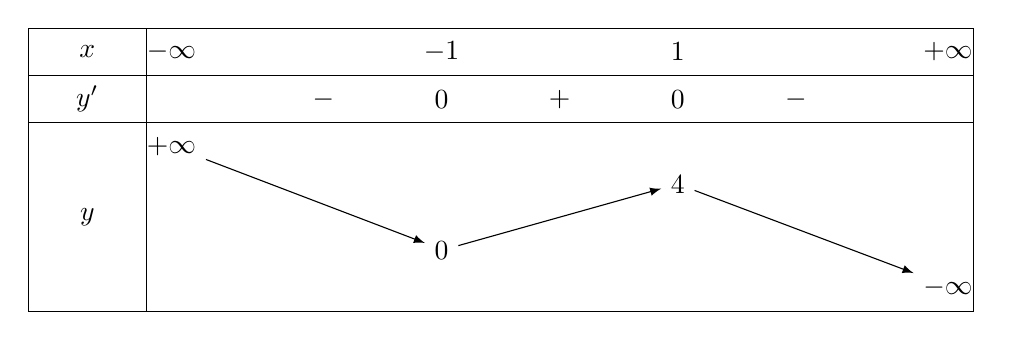
\begin{tikzpicture}[yscale=.6,xscale=1.5, kxd/.pic={\draw[double distance=1pt] (90:.3)--(-90:.3);}]
\path (0,0) node{$x$} ++(0:1) node[left=-.2]{$-\infty$} ++(0:2) node{$-1$} ++(0:2) node{$1$} ++(0:2)  node[right=-.2]{$+\infty$}
 (0,-1) node{$y'$} ++(0:2) node{$-$} ++(0:1) node{$0$} ++(0:1) node{$+$} ++(0:1) node{$0$} ++(0:1) node{$-$}
(0,-3.5) coordinate(a) node{$y$}
(1,-2) node[left=-.2] (A) {$+\infty$} (3,-4.2) node (B) {$0$} (5,-2.8) node (C) {$4$} (7,-5) node[right=-.2] (D) {$-\infty$};
\foreach \d/\dd in {A/B, B/C, C/D} \draw[-latex] ([shift={(45:.2)}]\d) -- ([shift={(-135:.2)}]\dd);
\begin{scope}[shift={(-.5,.5)}]
\draw (0,0) rectangle +(8,-6) (0,-1)--+(0:8) (0,-2)--+(0:8) (1,0)--+(-90:6);
\end{scope}
\end{tikzpicture}
}
Chọn khẳng định đúng.
\choice
{Hàm số $y=f(x)$ nghịch biến trên khoảng $(-1; 1)$}
{Hàm số $y=f(x)$ nghịch biến trên khoảng $(-1;+\infty)$}
{Hàm số $y=f(x)$ đồng biến trên khoảng $(-\infty ;-1)$}
{\True Hàm số $y=f(x)$ đồng biến trên khoảng $(-1; 1)$}
\loigiai
{
Dựa vào bảng biến thiên đã cho
\begin{itemize}
	\item Hàm số $y=f(x)$ đồng biến trên khoảng $(-1;1)$.
	\item Hàm số $y=f(x)$ nghịch biến trên mỗi khoảng $(-\infty;-1)$ và $(1;+\infty)$.
\end{itemize}
}
\end{ex}

\begin{ex}%[2D1N2-2]%[Tổ 1 - Đợt 16 - Chương 1 - Bài 1 - Cánh Diều]%[Cao Thành Thái]
Cho hàm số $y=f(x)$ có bảng biến thiên như sau:\\
\centerline
{
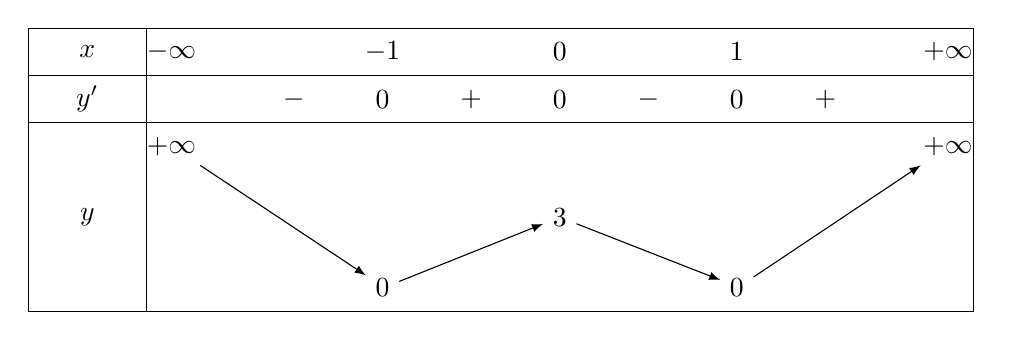
\begin{tikzpicture}[yscale=.6,xscale=1.5, kxd/.pic={\draw[double distance=1pt] (90:.3)--(-90:.3);}]
\path (0,0) node{$x$} ++(0:1) node[left=-.2]{$-\infty$} ++(0:1.5) node{$-1$} ++(0:1.5) node{$0$} ++(0:1.5) node{$1$} ++(0:1.5)  node[right=-.2]{$+\infty$}
(0,-1) node{$y'$} ++(0:1.75) node{$-$} ++(0:.75) node{$0$} ++(0:.75) node{$+$} ++(0:.75) node{$0$} ++(0:.75) node{$-$} ++(0:.75) node{$0$} ++(0:.75) node{$+$}
(0,-3.5) coordinate(a) node{$y$}
(1,-2) node[left=-.2] (A) {$+\infty$} (2.5,-5) node (B) {$0$} (4,-3.5) node (C) {$3$} (5.5,-5) node (D) {$0$} (7,-2) node[right=-.2] (E) {$+\infty$};
 \foreach \d/\dd in {A/B, B/C, C/D, D/E} \draw[-latex] ([shift={(45:.2)}]\d) -- ([shift={(-135:.2)}]\dd);
\begin{scope}[shift={(-.5,.5)}]
\draw (0,0) rectangle +(8,-6) (0,-1)--+(0:8) (0,-2)--+(0:8) (1,0)--+(-90:6);
\end{scope}
\end{tikzpicture}
}
Mệnh đề nào dưới đây \textbf{sai}?
\choice
{Hàm số $y=f(x)$ có hai điểm cực tiểu}
{\True Hàm số $y=f(x)$ có giá trị cực đại bằng $0$}
{Hàm số $y=f(x)$ có ba điểm cực trị}
{Hàm số $y=f(x)$ có giá trị cực đại bằng $3$}
\loigiai
{
Dựa vào bảng biến thiên đã cho
\begin{itemize}
	\item Hàm số $y=f(x)$ có hai điểm cực tiểu là $x=-1$, $x=1$; giá trị cực tiểu của hàm số $y=f(x)$ bằng $0$.
	\item Hàm số $y=f(x)$ có một điểm cực đại là $x=0$; giá trị cực đại của hàm số $y=f(x)$ bằng $3$.
\end{itemize}
}
\end{ex}

\begin{ex}%[2D1H1-2]%[Tổ 1 - Đợt 16 - Chương 1 - Bài 1 - Cánh Diều]%[Cao Thành Thái]
\immini
{
Cho hàm số $y=f(x)$ xác định, liên tục trên $\mathbb{R}$ và có đạo hàm $f'(x)$. Biết rằng hàm số $f'(x)$ có đồ thị như hình vẽ bên. Mệnh đề nào sau đây đúng?
\choice
{Hàm số $y=f(x)$ đồng biến trên khoảng $(-2; 0)$}
{\True Hàm số $y=f(x)$ nghịch biến trên khoảng $(0;+\infty)$}
{Hàm số $y=f(x)$ đồng biến trên khoảng $(-\infty ;-3)$}
{Hàm số $y=f(x)$ nghịch biến trên khoảng $(-3;-2)$}
}
{
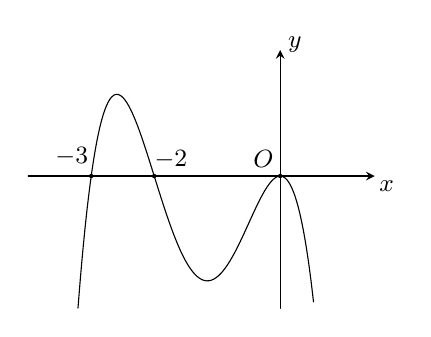
\begin{tikzpicture}[font=\small,line cap=round,line join=round,>=stealth, declare function={f(\x)=-.8*(\x)^2*(\x+3)*(\x+2);},scale=.8]
\draw[->] (-4,0)--(1.5,0) node[shift={(-40:.2)}]{$x$};
\draw[->] (0,-2.1)--(0,2) node[shift={(20:.2)}]{$y$};
\draw[samples=100,smooth,domain=-3.21:.53] plot (\x,{f(\x)});
\fill (0,0) circle(1pt) node[shift={(135:.3)}]{$O$} (-3,0) circle(1pt) node[shift={(135:.35)}]{$-3$} (-2,0) circle(1pt) node[shift={(45:.3)}]{$-2$};
\end{tikzpicture}
}
\loigiai
{
Dựa vào đồ thị của hàm số $y=f'(x)$ thì phương trình $f'(x)=0$ có ba nghiệm $x=-3$, $x=-2$, $x=0$.\\
Bảng biến thiên của hàm số $y=f(x)$\\
\centerline
{
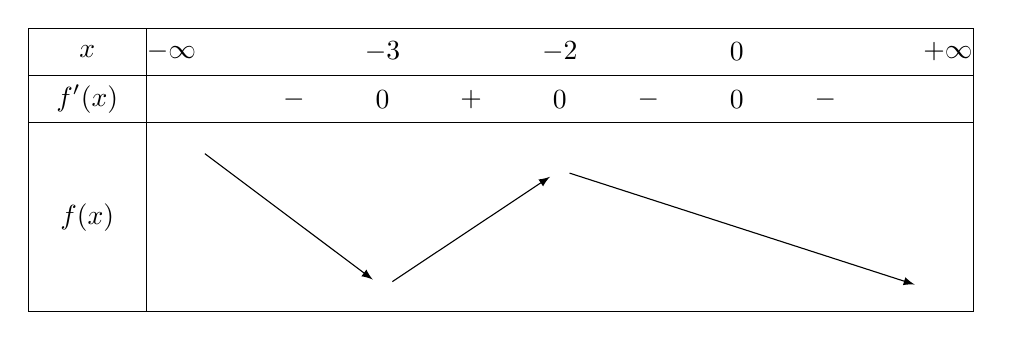
\begin{tikzpicture}[yscale=.6,xscale=1.5, kxd/.pic={\draw[double distance=1pt] (90:.3)--(-90:.3);}]
\path (0,0) node{$x$} ++(0:1) node[left=-.2]{$-\infty$} ++(0:1.5) node{$-3$} ++(0:1.5) node{$-2$} ++(0:1.5) node{$0$} ++(0:1.5)  node[right=-.2]{$+\infty$}
(0,-1) node{$f'(x)$} ++(0:1.75) node{$-$} ++(0:.75) node{$0$} ++(0:.75) node{$+$} ++(0:.75) node{$0$} ++(0:.75) node{$-$} ++(0:.75) node{$0$} ++(0:.75) node{$-$}
(0,-3.5) coordinate(a) node{$f(x)$}
(1,-2) node[left=.2] (A) {} (2.5,-5) node (B) {} (4,-2.5) node (C) {} (7,-5) node[right=.2] (D) {};
 \foreach \d/\dd in {A/B, B/C, C/D} \draw[-latex] ([shift={(45:.2)}]\d) -- ([shift={(-135:.2)}]\dd);
\begin{scope}[shift={(-.5,.5)}]
\draw (0,0) rectangle +(8,-6) (0,-1)--+(0:8) (0,-2)--+(0:8) (1,0)--+(-90:6);
\end{scope}
\end{tikzpicture}
}
Dựa vào bảng biến thiên trên, hàm số $y=f(x)$ nghịch biến trên mỗi khoảng $(-\infty;-3)$ và $(-2;+\infty)$; đồng biến trên khoảng $(-3;-2)$.\\
Vậy hàm số $y=f(x)$ cũng nghịch biến trên khoảng $(0;+\infty)$.
}
\end{ex}

\begin{ex}%[2D1H2-2]%[Tổ 1 - Đợt 16 - Chương 1 - Bài 1 - Cánh Diều]%[Cao Thành Thái]
Cho hàm số $y=f(x)$ liên tục trên $\mathbb{R}$ và có bảng xét dấu của đạo hàm như sau:\\
\centerline
{
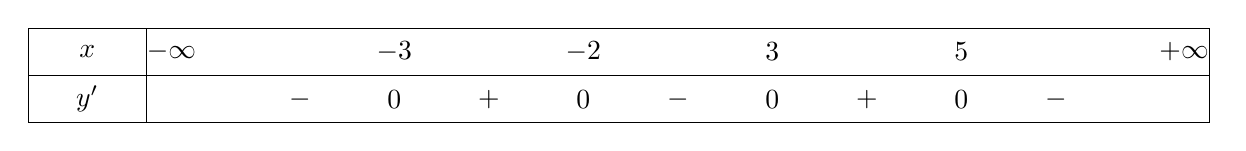
\begin{tikzpicture}[yscale=.6,xscale=1.5, kxd/.pic={\draw[double distance=1pt] (90:.3)--(-90:.3);}]
\path (0,0) node{$x$} ++(0:1) node[left=-.2]{$-\infty$} ++(0:1.6) node{$-3$} ++(0:1.6) node{$-2$} ++(0:1.6) node{$3$} ++(0:1.6) node{$5$} ++(0:1.6)  node[right=-.2]{$+\infty$}
(0,-1) node{$y'$} ++(0:1.8) node{$-$} ++(0:.8) node{$0$} ++(0:.8) node{$+$} ++(0:.8) node{$0$} ++(0:.8) node{$-$} ++(0:.8) node{$0$} ++(0:.8) node{$+$} ++(0:.8) node{$0$} ++(0:.8) node{$-$};
\begin{scope}[shift={(-.5,.5)}]
\draw (0,0) rectangle +(10,-2) (0,-1)--+(0:10) (1,0)--+(-90:2);
\end{scope}
\end{tikzpicture}
}
Số điểm cực trị của hàm số đã cho là
\choice
{$5$}
{$3$}
{$2$}
{\True $4$}
\loigiai
{
Vì dấu của $y'$ thay đổi từ âm sang dương khi qua các điểm $x=-3$, $x=3$ theo chiều tăng của $x$ nên hàm số $y=f(x)$ đạt cực tiểu tại các điểm $x=-3$, $x=3$.\\
Vì dấu của $y'$ thay đổi từ dương sang âm khi qua các điểm $x=-2$, $x=5$ theo chiều tăng của $x$ nên hàm số $y=f(x)$ đạt cực đại tại các điểm $x=-2$, $x=5$.\\
Vậy hàm số $y=f(x)$ có $4$ điểm cực trị.
}
\end{ex}

\begin{ex}%[2D1H1-1]%[Tổ 1 - Đợt 16 - Chương 1 - Bài 1 - Cánh Diều]%[Cao Thành Thái]
Hàm số $y=2x^3-6x-3$ nghịch biến trên khoảng nào?
\choice
{$(-\infty;+\infty)$}
{$(1;+\infty)$}
{$(-\infty ;-1)$}
{\True $(-1; 1)$}
\loigiai
{
Hàm số $y=2x^3-6x-3$ có tập xác định là $\mathscr{D} = \mathbb{R}$.\\
Đạo hàm $y' = 6x^2-6$. Khi đó, phương trình $y'=0$ có hai nghiệm phân biệt $x=-1$, $x=1$.\\
Thêm nữa, $\lim\limits_{x\to -\infty} y = -\infty$ và $\lim\limits_{x\to +\infty} y = +\infty$.\\
Bảng biến thiên\\
\centerline
{
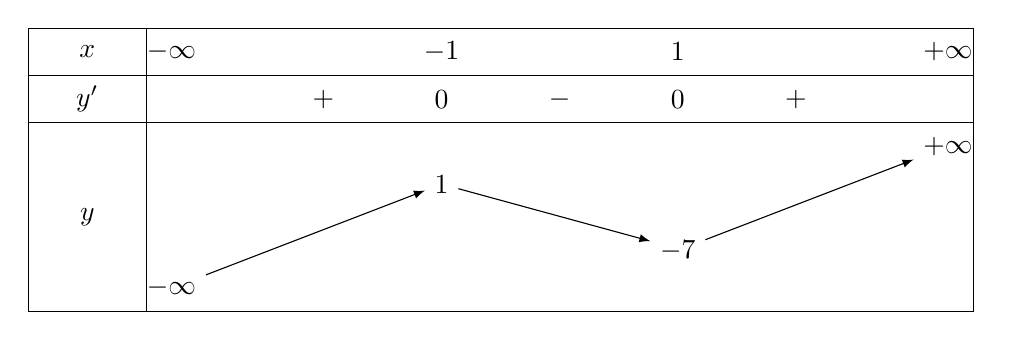
\begin{tikzpicture}[yscale=.6,xscale=1.5, kxd/.pic={\draw[double distance=1pt] (90:.3)--(-90:.3);}]
\path (0,0) node{$x$} ++(0:1) node[left=-.2]{$-\infty$} ++(0:2) node{$-1$} ++(0:2) node{$1$} ++(0:2)  node[right=-.2]{$+\infty$}
 (0,-1) node{$y'$} ++(0:2) node{$+$} ++(0:1) node{$0$} ++(0:1) node{$-$} ++(0:1) node{$0$} ++(0:1) node{$+$}
(0,-3.5) coordinate(a) node{$y$}
(1,-5) node[left=-.2] (A) {$-\infty$} (3,-2.8) node (B) {$1$} (5,-4.2) node (C) {$-7$} (7,-2) node[right=-.2] (D) {$+\infty$};
\foreach \d/\dd in {A/B, B/C, C/D} \draw[-latex] ([shift={(45:.2)}]\d) -- ([shift={(-135:.2)}]\dd);
\begin{scope}[shift={(-.5,.5)}]
\draw (0,0) rectangle +(8,-6) (0,-1)--+(0:8) (0,-2)--+(0:8) (1,0)--+(-90:6);
\end{scope}
\end{tikzpicture}
}
Vậy hàm số $y=2x^3-6x-3$ nghịch biến trên khoảng $(-1;1)$; đồng biến trên mỗi khoảng $(-\infty;-1)$ và $(1;+\infty)$.
}
\end{ex}

\begin{ex}%[2D1H1-1]%[Tổ 1 - Đợt 16 - Chương 1 - Bài 1 - Cánh Diều]%[Cao Thành Thái]
Hàm số $y=\dfrac{2x-1}{x+2}$ đồng biến trên khoảng nào?
\choice
{\True $(-\infty ;-2)$, $(-2;+\infty)$}
{$(-\infty ;-1)$}
{$(-4;+\infty)$}
{$\mathbb{R} \setminus\{-2\}$}
\loigiai
{
Hàm số $y=\dfrac{2x-1}{x+2}$ có tập xác định là $\mathscr{D} = \mathbb{R}\setminus \{-2\}$.\\
Đạo hàm $y'=\dfrac{5}{(x+2)^2}>0, \forall x\neq -2$.\\
Vậy hàm số $y=\dfrac{2x-1}{x+2}$ đồng biến trên mỗi khoảng $(-\infty;-2)$ và $(-2;+\infty)$.
}
\end{ex}

\begin{ex}%[2D1H1-1]%[Tổ 1 - Đợt 16 - Chương 1 - Bài 1 - Cánh Diều]%[Cao Thành Thái]
Hàm số $y=\sqrt{4-x^2}$ đồng biến trên khoảng nào?
\choice
{$(-2;+\infty)$}
{$(0; 2)$}
{$(-2; 2)$}
{\True $(-2; 0)$}
\loigiai
{
Hàm số $y=\sqrt{4-x^2}$ có tập xác định là $\mathscr{D} = [-2;2]$.\\
Đạo hàm $y'=\dfrac{\left(4-x^2\right)'}{2\sqrt{4-x^2}} = \dfrac{-x}{\sqrt{4-x^2}}, \forall x\in (-2;2)$.\\
Khi đó,
\[y'=0 \Leftrightarrow \dfrac{-x}{\sqrt{4-x^2}} = 0 \Leftrightarrow x=0.\]
Bảng biến thiên\\
\centerline
{
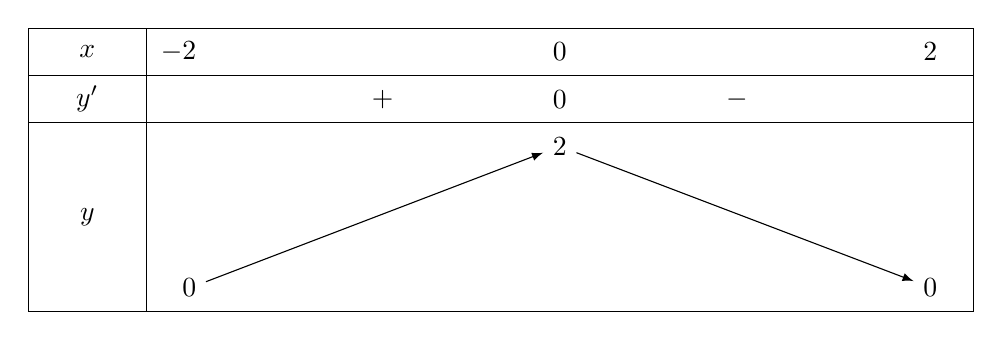
\begin{tikzpicture}[yscale=.6,xscale=1.5, kxd/.pic={\draw[double distance=1pt] (90:.3)--(-90:.3);}]
\path (0,0) node{$x$} ++(0:1) node[left=-.2]{$-2$} ++(0:3) node{$0$} ++(0:3) node[right=-.2]{$2$}
(0,-1) node{$y'$} ++(0:2.5) node{$+$} ++(0:1.5) node{$0$} ++(0:1.5) node{$-$}
(0,-3.5) coordinate(a) node{$y$}
(1,-5) node[left=-.2] (A) {$0$} (4,-2) node (B) {$2$} (7,-5) node[right=-.2] (C) {$0$};
\foreach \d/\dd in {A/B, B/C} \draw[-latex] ([shift={(45:.2)}]\d) -- ([shift={(-135:.2)}]\dd);
\begin{scope}[shift={(-.5,.5)}]
\draw (0,0) rectangle +(8,-6) (0,-1)--+(0:8) (0,-2)--+(0:8) (1,0)--+(-90:6);
\end{scope}
\end{tikzpicture}
}
Vậy hàm số $y=\sqrt{4-x^2}$ đồng biến trên khoảng $(-2;0)$; nghịch biến trên khoảng $(0;2)$.
}
\end{ex}

\begin{ex}%[2D1H2-1]%[Tổ 1 - Đợt 16 - Chương 1 - Bài 1 - Cánh Diều]%[Cao Thành Thái]
Hàm số $y=-x^3+4x^2-5x+1$ có điểm cực đại là $x=a$ và giá trị cực tiểu là $y=b$. Tính $a-b$.
\choice
{$\dfrac{24}{27}$}
{$0$}
{$\dfrac{68}{27}$}
{\True $\dfrac{8}{3}$}
\loigiai
{
Hàm số $y=-x^3+4x^2-5x+1$ có tập xác định là $\mathscr{D} = \mathbb{R}$.\\
Đạo hàm $y'=-3x^2+8x-5$.\\
Khi đó,
\[y'=0 \Leftrightarrow -3x^2+8x-5=0 \Leftrightarrow \hoac{&x=1 \\&x=\dfrac{5}{3}.}\]
Thêm nữa, $\lim\limits_{x\to -\infty} y = +\infty$ và $\lim\limits_{x\to +\infty} y = -\infty$.\\
Bảng biến thiên\\
\centerline
{
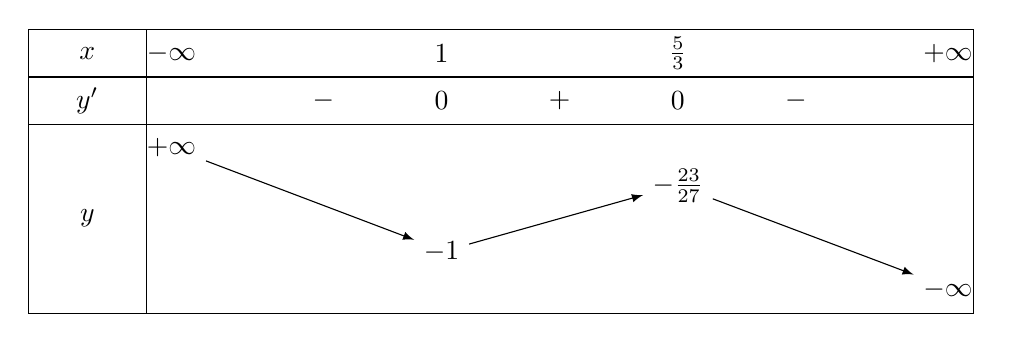
\begin{tikzpicture}[yscale=.6,xscale=1.5, kxd/.pic={\draw[double distance=1pt] (90:.3)--(-90:.3);}]
\path (0,0) node{$x$} ++(0:1) node[left=-.2]{$-\infty$} ++(0:2) node{$1$} ++(0:2) node{$\frac{5}{3}$} ++(0:2)  node[right=-.2]{$+\infty$}
 (0,-1) node{$y'$} ++(0:2) node{$-$} ++(0:1) node{$0$} ++(0:1) node{$+$} ++(0:1) node{$0$} ++(0:1) node{$-$}
(0,-3.5) coordinate(a) node{$y$}
(1,-2) node[left=-.2] (A) {$+\infty$} (3,-4.2) node (B) {$-1$} (5,-2.8) node (C) {$-\frac{23}{27}$} (7,-5) node[right=-.2] (D) {$-\infty$};
\foreach \d/\dd in {A/B, B/C, C/D} \draw[-latex] ([shift={(45:.2)}]\d) -- ([shift={(-135:.2)}]\dd);
\begin{scope}[shift={(-.5,.5)}]
\draw (0,0) rectangle +(8,-6) (0,-1)--+(0:8) (0,-2)--+(0:8) (1,0)--+(-90:6);
\end{scope}
\end{tikzpicture}
}
Dựa vào bảng biến thiên trên, hàm số $y=-x^3+4x^2-5x+1$ có điểm cực đại là $x=\dfrac{5}{3}$ và giá trị cực tiểu của nó bằng $-1$.\\
Suy ra $a=\dfrac{5}{3}$ và $b=-1$.\\
Vậy $a-b = \dfrac{5}{3}-(-1) = \dfrac{8}{3}$.
}
\end{ex}

\begin{ex}%[2D1H2-1]%[Tổ 1 - Đợt 16 - Chương 1 - Bài 1 - Cánh Diều]%[Cao Thành Thái]
Cho hàm số $y=f(x)$ có đạo hàm $f'(x)=\left(x^2-4\right)(3-x)(x+2), \forall x \in \mathbb{R}$. Số điểm cực trị của hàm số đã cho là
\choice
{\True $2$}
{$1$}
{$3$}
{$4$}
\loigiai
{
Ta có
\[f'(x) = 0 \Leftrightarrow \left(x^2-4\right)(3-x)(x+2)=0 \Leftrightarrow \hoac{&x^2-4=0 \\&3-x=0 \\&x+2=0} \Leftrightarrow \hoac{&x=-2\,(\text{nghiệm bội chẵn}) \\&x=2\,(\text{nghiệm đơn}) \\&x=3\,(\text{nghiệm đơn}).}\]
Lại có $\lim\limits_{x\to +\infty} f'(x) = -\infty$.\\
Bảng biến thiên của hàm số $y=f(x)$\\
\centerline
{
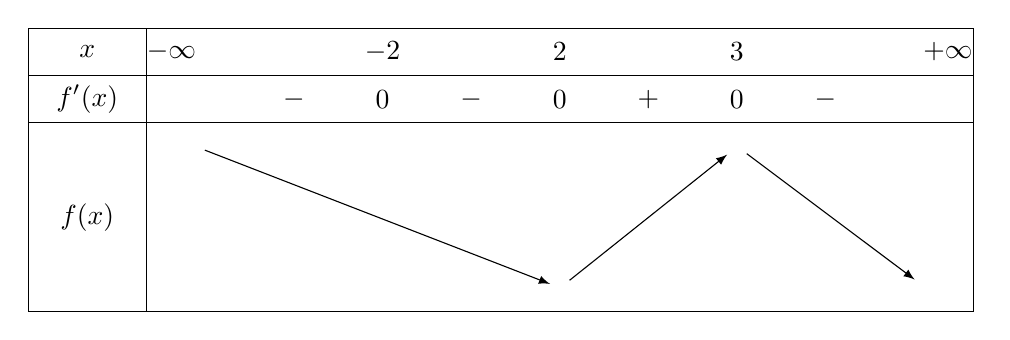
\begin{tikzpicture}[yscale=.6,xscale=1.5, kxd/.pic={\draw[double distance=1pt] (90:.3)--(-90:.3);}]
\path (0,0) node{$x$} ++(0:1) node[left=-.2]{$-\infty$} ++(0:1.5) node{$-2$} ++(0:1.5) node{$2$} ++(0:1.5) node{$3$} ++(0:1.5)  node[right=-.2]{$+\infty$}
(0,-1) node{$f'(x)$} ++(0:1.75) node{$-$} ++(0:.75) node{$0$} ++(0:.75) node{$-$} ++(0:.75) node{$0$} ++(0:.75) node{$+$} ++(0:.75) node{$0$} ++(0:.75) node{$-$}
(0,-3.5) coordinate(a) node{$f(x)$}
(1,-2) node[left=.2] (A) {} (4,-5) node (B) {} (5.5,-2) node (C) {} (7,-5) node[right=.2] (D) {};
 \foreach \d/\dd in {A/B, B/C, C/D} \draw[-latex] ([shift={(45:.2)}]\d) -- ([shift={(-135:.2)}]\dd);
\begin{scope}[shift={(-.5,.5)}]
\draw (0,0) rectangle +(8,-6) (0,-1)--+(0:8) (0,-2)--+(0:8) (1,0)--+(-90:6);
\end{scope}
\end{tikzpicture}
}
Vậy hàm số $y=f(x)$ có $2$ điểm cực trị.
}
\end{ex}

\begin{ex}%[2D1H1-1]%[Tổ 1 - Đợt 16 - Chương 1 - Bài 1 - Cánh Diều]%[Cao Thành Thái]
Hàm số $f(x)=3^{x^2-2x}$ đồng biến trên khoảng nào sau đây?
\choice
{\True $(1;+\infty)$}
{$(0; 2)$}
{$(-\infty ; 0)$}
{$(0;+\infty)$}
\loigiai
{
Hàm số $f(x)=3^{x^2-2x}$ có tập xác định là $\mathscr{D} = \mathbb{R}$.\\
Đạo hàm $f'(x) = \left(x^2-2x\right)'\cdot 3^{x^2-2x} \ln 3= (2x-2) 3^{x^2-2x}\ln 3$.\\
Khi đó,
\[f'(x)=0 \Leftrightarrow (2x-2) 3^{x^2-2x}\ln 3 = 0 \Leftrightarrow 2x-2 = 0 \Leftrightarrow x=1.\]
Thêm nữa, $\lim\limits_{x\to -\infty} y = +\infty$ và $\lim\limits_{x\to +\infty} y = +\infty$.\\
Bảng biến thiên\\
\centerline
{
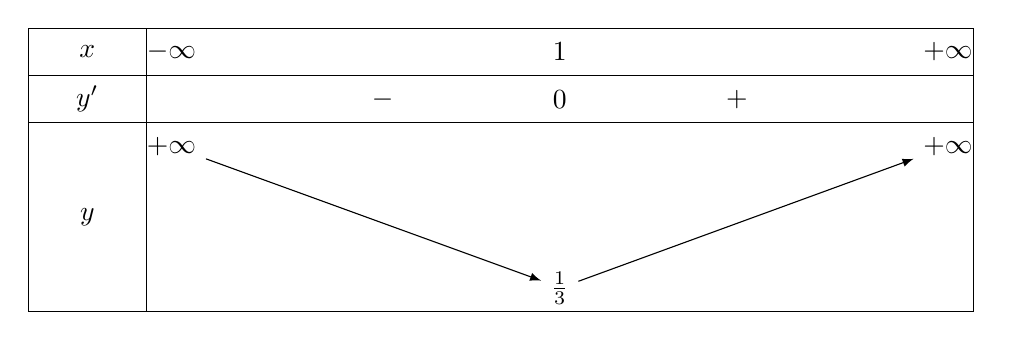
\begin{tikzpicture}[yscale=.6,xscale=1.5, kxd/.pic={\draw[double distance=1pt] (90:.3)--(-90:.3);}]
\path (0,0) node{$x$} ++(0:1) node[left=-.2]{$-\infty$} ++(0:3) node{$1$} ++(0:3) node[right=-.2]{$+\infty$}
(0,-1) node{$y'$} ++(0:2.5) node{$-$} ++(0:1.5) node{$0$} ++(0:1.5) node{$+$}
(0,-3.5) coordinate(a) node{$y$}
(1,-2) node[left=-.2] (A) {$+\infty$} (4,-5) node (B) {$\frac{1}{3}$} (7,-2) node[right=-.2] (C) {$+\infty$};
\foreach \d/\dd in {A/B, B/C} \draw[-latex] ([shift={(45:.2)}]\d) -- ([shift={(-135:.2)}]\dd);
\begin{scope}[shift={(-.5,.5)}]
\draw (0,0) rectangle +(8,-6) (0,-1)--+(0:8) (0,-2)--+(0:8) (1,0)--+(-90:6);
\end{scope}
\end{tikzpicture}
}
Vậy hàm số $f(x)=3^{x^2-2x}$ đồng biến trên khoảng $(1;+\infty)$; nghịch biến trên khoảng $(-\infty;1)$.
}
\end{ex}

\begin{ex}%[2D1H1-1]%[Tổ 1 - Đợt 16 - Chương 1 - Bài 1 - Cánh Diều]%[Cao Thành Thái]
Hàm số $f(x)=\log_{\frac{\sqrt{2}}{2}}(4x-3)$ nghịch biến trên khoảng nào sau đây?
\choice
{$(-\infty ;+\infty)$}
{\True $(1;+\infty)$}
{$\left(-\infty ; \dfrac{3}{4}\right)$}
{$\left(0; \dfrac{3}{4}\right)$}
\loigiai
{
Hàm số $f(x)=\log_{\frac{\sqrt{2}}{2}}(4x-3)$ có tập xác định là $\mathscr{D} = \left(\dfrac{3}{4}; +\infty\right)$.\\
Đạo hàm $f'(x) = \dfrac{(4x-3)'}{(4x-3)\ln\dfrac{\sqrt{2}}{2}} = \dfrac{-8}{(4x-3)\ln 2}<0, \forall x\in \left(\dfrac{3}{4};+\infty\right)$.\\
Vậy hàm số $f(x)=\log_{\frac{\sqrt{2}}{2}}(4x-3)$ nghịch biến trên khoảng $\left(\dfrac{3}{4};+\infty\right)$.\\
Do đó, hàm số $f(x)=\log_{\frac{\sqrt{2}}{2}}(4x-3)$ cũng nghịch biến trên khoảng $(1;+\infty)$.
}
\end{ex}

\begin{ex}%[2D1V1-3]%[Tổ 1 - Đợt 16 - Chương 1 - Bài 1 - Cánh Diều]%[Cao Thành Thái]
Có bao nhiêu giá trị nguyên của tham số $m$ thuộc khoảng $(-2024; 2026)$ để hàm số $f(x)=\dfrac{1}{3}x^3+mx^2+9x-3$ đồng biến trên $\mathbb{R}$?
\choice
{$6$}
{\True $7$}
{$4046$}
{$4044$}
\loigiai
{
Hàm số $f(x)=\dfrac{1}{3}x^3+mx^2+9x-3$ có tập xác định là $\mathscr{D} = \mathbb{R}$.\\
Đạo hàm $f'(x) = x^2+2mx+9$.\\
Hàm số $f(x)=\dfrac{1}{3}x^3+mx^2+9x-3$ đồng biến trên $\mathbb{R}$ khi và chỉ khi
\[f'(x)\geq 0, \forall x\in\mathbb{R} \Leftrightarrow x^2+2mx+9\geq 0, \forall x\in \mathbb{R} \Leftrightarrow m^2-9\leq 0 \Leftrightarrow -3\leq m\leq 3.\]
Vì $m\in\mathbb{Z}$, $m\in (-2024;2026)$ và thỏa mãn $-3\leq m\leq 3$ nên $m\in \{-3;-2;-1;0;1;2;3\}$.\\
Vậy có tất cả $7$ giá trị nguyên của $m$ thỏa mãn yêu cầu bài toán.
}
\end{ex}
\begin{ex}%[2D1H3-2] 
Cho hàm số $y=\dfrac{x^2+4}{x}$, khi đó giá trị nhỏ nhất của hàm số trên khoảng $\left(0;+\infty\right)$ đạt được tại điểm nào? 
\choice
{$x=1$}
{$x=4$}
{$x=3$}
{\True $x=2$}
\loigiai{
Xét hàm số $f(x)=\dfrac{x^2+4}{x}$ với $ x\in\left(0;+\infty\right)$.\\
Ta có $f'(x)=\dfrac{x^2-4}{x^2}$. Khi đó $f'(x)=0\Rightarrow x=2$.\\
Ngoài ra $\lim\limits_{x\to{0^+}}f(x)=+\infty ,\,\lim\limits_{x\to+\infty}f(x)=+\infty$.\\
Ta có bảng biến thiên hàm số như sau
\begin{center}
	
\begin{tikzpicture}
			\tkzTabInit[lgt=1.2,espcl=4]
			{$x$/1,$f’(x)$/1,$f(x)$/2}
			{$0$,$2$,$+\infty$}
			\tkzTabLine{ ,-,z,+, }
			\tkzTabVar{+/$+\infty$,-/$4$,+/$+\infty$}
		\end{tikzpicture}
\end{center}
Vậy hàm số đạt giá trị nhỏ nhất trên khoảng $\left(0;+\infty\right)$ bằng $4$ tại điểm $x=2$.}
\end{ex}

\begin{ex}%[2D1H3-1] 
Giá trị lớn nhất hàm số $y=x^4-4x^2+5$ trên $\left[-2;3\right]$ là
\choice
{$122$}
{$1$}
{$5$}
{\True $50$}
\loigiai{
Ta có $y'=4x^3-8x$; $y'=0\Leftrightarrow 4x^3-8x=0\Leftrightarrow\hoac{&
x=0\\&
x=\sqrt 2\\&
x=-\sqrt 2.}$\\
Do $f(\sqrt 2)=1\,;f(-\sqrt 2)=1\,;\,f(0)=5\,;\,f(-2)=5\,;\,f(3)=50$.\\
Suy ra giá trị lớn nhất của hàm số $y=x^4-4x^2+5$ trên $\left[-2;3\right]$ là $50$ tại $x=3$.}
\end{ex}

\begin{ex}%[2D1N3-1] 
\immini{
Cho hàm số $y=f(x)$ liên tục trên đoạn $\left[-1;3\right]$ và có đồ thị như hình vẽ. Giá trị lớn nhất của hàm số đã cho trên đoạn $\left[-1;3\right]$ bằng
\choice
{\True $3$}
{$2$}
{$0$}
{$1$}}
{	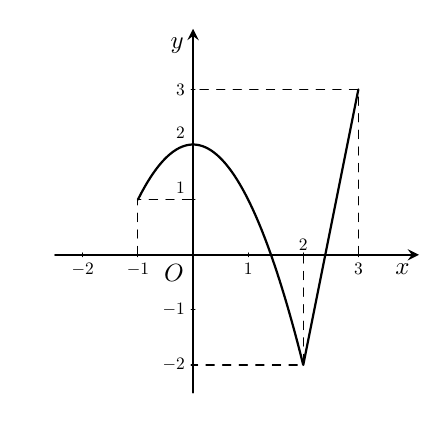
\begin{tikzpicture}[line join=round, line cap=round,>=stealth,thick,scale=.7]
		\tikzset{every node/.style={scale=0.9}}
		\draw[->] (-2.5,0)--(4.1,0) node[below left] {$x$};
		\draw[->] (0,-2.5)--(0,4.1) node[below left] {$y$};
		\draw (0,0) node [below left] {$O$};
		\foreach \x/\nx in {-2/-2,-1/-1,1/1,3/3}
		\draw[thin] (\x,1pt)--(\x,-1pt) node [scale=.7,below] {$\nx$};
		\foreach \x/\nx in {2/2}
		\draw[thin] (\x,1pt)--(\x,-1pt) node [scale=.7,above] {$\nx$};
		\foreach \y/\ny in {-2/-2,-1/-1,3/3}
		\draw[thin] (1pt,\y)--(-1pt,\y) node[scale=.7,left] {$\ny$};
			\foreach \y/\ny in {1/1,2/2}
		\draw[thin] (1pt,\y)--(-1pt,\y) node [scale=.7,above left] {$\ny$};
		\draw[dashed,thin](-1,0)--(-1,1)--(0,1);
		\draw[dashed,thin](2,0)--(2,-2)--(0,-2);
		\draw[dashed,thin](3,0)--(3,3)--(0,3);
		\begin{scope}
			\clip (-3,-3) rectangle (4,4);
			\draw[samples=200,domain=-1:2,smooth,variable=\x] plot (\x,{-1*(\x)^2+0*(\x)+2});
		\end{scope}
	\draw (2,-2)--(3,3);
	\end{tikzpicture}}
\loigiai{
Xét hàm số $y=f(x)$ trên đoạn $\left[-1;\,3\right]$. Dựa vào đồ thị ta có $\max\limits_{\left[-1;3\right]}f(x)=f(3)=3$.}
\end{ex}

\begin{ex}%[2D1N3-1] 
\immini{
Cho hàm số $y=f(x)$ xác định và liên tục trên có đồ thị như hình bên. Gọi $M,m$ lần lượt là giá trị lớn nhất và nhỏ nhất của hàm số trên đoạn $[1;3].$ Giá trị của $M+m$ bằng
\choice
{$M+m=2$}
{\True $M+m=-4$}
{$M+m=-3$}
{$M+m=1$}}
{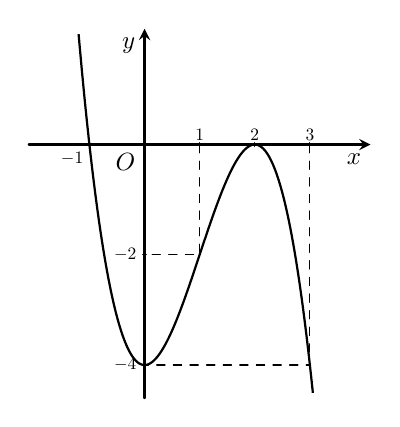
\begin{tikzpicture}[line join=round, line cap=round,>=stealth,thick, scale=.7]
	\tikzset{every node/.style={scale=0.9}}
	\draw[->] (-2.1,0)--(4.1,0) node[below left] {$x$};
	\draw[->] (0,-4.6)--(0,2.1) node[below left] {$y$};
	\draw (0,0) node [below left] {$O$};
	\foreach \x/\nx in {1/1,2/2,3/3}
	\draw[thin] (\x,1pt)--(\x,-1pt) node [scale=.7,above] {$\nx$};
		\foreach \x/\nx in {-1/-1}
	\draw[thin] (\x,1pt)--(\x,-1pt) node [scale=.7,below left] {$\nx$};
	\foreach \y/\ny in {-4/-4,-2/-2}
	\draw[thin] (1pt,\y)--(-1pt,\y) node [scale=.7,left] {$\ny$};
	\draw[dashed,thin](1,0)--(1,-2)--(0,-2);
	\draw[dashed,thin](3,0)--(3,-4)--(0,-4);
	\begin{scope}
		\clip (-2,-4.5) rectangle (4,2);
		\draw[samples=200,domain=-1.2:3.1,smooth,variable=\x] plot(\x,{0-((\x)+1.0)*((\x)-2.0)^(2.0)});
	\end{scope}
\end{tikzpicture}}
\loigiai{
Dựa vào đồ thị hàm số, ta được $\heva{&
M=0\\&
m=-4}\Rightarrow M+m=-4$.}
\end{ex}

\begin{ex}%[2D1V3-1] 
\immini{
Cho hàm số $y=f(x)$ liên tục trên $[-2;3]$ và có đồ thị như hình vẽ bên dưới. Gọi $M$ và $m$ lần lượt là giá trị lớn nhất và nhỏ nhất của hàm số $y=f(2\cos 5x+1).$ Giá trị của $M-2m$ bằng bao nhiêu?
\choice
{\True $M-2m=5$}
{$M-2m=3$}
{$M-2m=6$}
{$M-2m=7$}}
{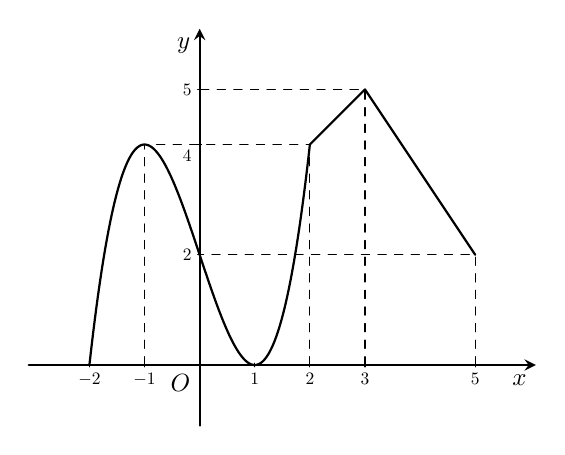
\begin{tikzpicture}[line join=round, line cap=round,>=stealth,thick, scale=.7]
	\tikzset{every node/.style={scale=0.9}}
	\draw[->] (-3.1,0)--(6.1,0) node[below left] {$x$};
	\draw[->] (0,-1.1)--(0,6.1) node[below left] {$y$};
	\draw (0,0) node [below left] {$O$};
	\foreach \x/\nx in {-2/-2,-1/-1,1/1,2/2,3/3,5/5}
	\draw[thin] (\x,1pt)--(\x,-1pt) node [scale=.7,below] {$\nx$};
	\foreach \y/\ny in {2/2,5/5}
	\draw[thin] (1pt,\y)--(-1pt,\y) node [scale=.7,left] {$\ny$};
	\foreach \y/\ny in {4/4}
	\draw[thin] (1pt,\y)--(-1pt,\y) node [scale=.7,below left] {$\ny$};
	\draw[dashed,thin](-1,0)--(-1,4)--(0,4);
	\draw[dashed,thin](2,0)--(2,4)--(0,4);
	\draw[dashed,thin](3,0)--(3,5)--(0,5);
	\draw[dashed,thin](5,0)--(5,2)--(0,2);
	\begin{scope}
		\clip (-3,-1) rectangle (6,6);
		\draw[samples=200,domain=-2:2,smooth,variable=\x] plot(\x,{((\x)+2.0)*((\x)-1.0)^(2.0)});
	\end{scope}
\draw (2,4)--(3,5)--(5,2);
\end{tikzpicture}}
\loigiai{ 
Ta có $-1\le\cos 5x\le 1\Rightarrow -2\le 2\cos 5x\le 2\Rightarrow-1\le 2\cos 5x+1\le 3$.\\
Đặt $t=2\cos 5x+1$ với $x\in\left[-2;3\right]$ thì $t\in\left[-1;3\right]$.\\
Khi đó  $y=f\left(2\cos 5x+1\right)=f(t)$ với $t\in\left[-1;3\right]$.\\
Suy ra $\heva{&	
M=5\\&
m=0
}\Rightarrow M-2m=5.$}
\end{ex}

\begin{ex}%[2D1N3-1] 
Cho hàm số $y=f(x)$ liên tục trên $\mathbb{R}$ và có bảng biến thiên như hình dưới đây
\begin{center}
	
\begin{tikzpicture}
		\tkzTabInit[lgt=1.2,espcl=2]
		{$x$/.8,$f’(x)$/.8,$f(x)$/2}
		{$-\infty$,$-1$,$1$,$2$,$+\infty$}
		\tkzTabLine{ ,-,d,+,z,+,d,-, }
		\tkzTabVar{+/$+\infty$,-/$-3$,R/, +/$2$,-/$-4$}
	\end{tikzpicture}
\end{center}
Trong các mệnh đề sau, mệnh đề nào {\bf sai}?
\choice
{Giá trị lớn nhất của hàm số $y=f(x)$ trên đoạn $\left[-1;\,2\right]$ bằng $2$}
{Giá trị nhỏ nhất của hàm số $y=f(x)$ trên đoạn $\left[-1;\,2\right]$ bằng $-3$}
{\True Giá trị nhỏ nhất của hàm số $y=f(x)$ trên nửa khoảng $\left[-1;\,+\infty\right)$ bằng $-4$}
{Giá trị lớn nhất của hàm số $y=f(x)$ trên nửa khoảng $\left[-1;\,+\infty\right)$ bằng $2$}
\loigiai{ 
Từ bảng biến thiên của hàm số $y=f(x)$ ta có $\lim\limits_{x\to+\infty}f(x)=-4$.\\ Suy ra không tồn tại giá trị nhỏ nhất của hàm số $f(x)$ trên nửa khoảng $\left[-1;\,+\infty\right)$.}
\end{ex}

\begin{ex}%[2D1N3-1] 
Cho hàm số $y=f(x)$ liên tục trên $\left[-3;2\right]$ và có bảng biến thiên như hình dưới
\begin{center}
	
\begin{tikzpicture}
		\tkzTabInit[lgt=1.2,espcl=2]
		{$x$/.7,$f’(x)$/.7,$f(x)$/2}
		{$-3$,$-1$,$0$,$1$,$2$}
		\tkzTabLine{ ,+,z,-,z,+,z,-, }
		\tkzTabVar{-/$-2$,+/$3$,-/$0$,+/$2$,-/$1$}
	\end{tikzpicture}
\end{center}
 Gọi $M,\,m$ lần lượt là giá trị lớn nhất và giá trị nhỏ nhất của hàm số $y=f(x)$ trên đoạn $\left[-1;\,2\right]$. Tính $2M+3m$.
\choice
{$2M+3m=0$}
{\True $2M+3m=6$}
{$2M+3m=-2$}
{$2M+3m=8$}
\loigiai{ 
Trên đoạn $\left[-1;\,2\right]$, giá trị lớn nhất của hàm số là $M=3$, giá trị nhỏ nhất của hàm số là $m=0$.\\
 Vậy $2M+3m=6$.}
\end{ex}

\begin{ex}%[2D1V3-1] 
\immini{
Cho hàm số $y=f(x)$ xác định và liên tục trên R, có đồ thị trên đoạn$\left[-1;\,3\right]$ như hình vẽ.
Tìm giá trị lớn nhất $M$ của hàm số $y=g(x)=f\left(\sin x+1\right)$ trên $\mathbb{R}$.
\choice
{$M=3$}
{$M=0$}
{$M=1$}
{\True $M=2$}}
{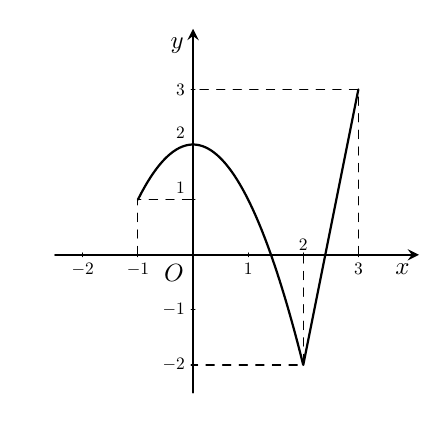
\begin{tikzpicture}[line join=round, line cap=round,>=stealth,thick,scale=.7]
		\tikzset{every node/.style={scale=0.9}}
		\draw[->] (-2.5,0)--(4.1,0) node[below left] {$x$};
		\draw[->] (0,-2.5)--(0,4.1) node[below left] {$y$};
		\draw (0,0) node [below left] {$O$};
		\foreach \x/\nx in {-2/-2,-1/-1,1/1,3/3}
		\draw[thin] (\x,1pt)--(\x,-1pt) node [scale=.7,below] {$\nx$};
		\foreach \x/\nx in {2/2}
		\draw[thin] (\x,1pt)--(\x,-1pt) node [scale=.7,above] {$\nx$};
		\foreach \y/\ny in {-2/-2,-1/-1,3/3}
		\draw[thin] (1pt,\y)--(-1pt,\y) node[scale=.7,left] {$\ny$};
			\foreach \y/\ny in {1/1,2/2}
		\draw[thin] (1pt,\y)--(-1pt,\y) node [scale=.7,above left] {$\ny$};
		\draw[dashed,thin](-1,0)--(-1,1)--(0,1);
		\draw[dashed,thin](2,0)--(2,-2)--(0,-2);
		\draw[dashed,thin](3,0)--(3,3)--(0,3);
		\begin{scope}
			\clip (-3,-3) rectangle (4,4);
			\draw[samples=200,domain=-1:2,smooth,variable=\x] plot (\x,{-1*(\x)^2+0*(\x)+2});
		\end{scope}
	\draw (2,-2)--(3,3);
	\end{tikzpicture}}
\loigiai{
Đặt $t=\sin x+1$ thì $t\in [0; 2]$.\\
Xét hàm số $y=f(t),\,\,t\in\left[0;\,2\right]$.\\
 Từ đồ thị đã cho ta có $M=\max\limits_{\left[0;2\right]}f(t)=f(0)=2.$}
\end{ex}

\begin{ex}%[2D1H3-1] 
Giá trị lớn nhất của hàm số $f(x)=\left|x^3-3x^2-1\right|$ trên đoạn $\left[-1;3\right]$ là
\choice
{$1$}
{$3$}
{$2$}
{\True $5$}
\loigiai{ 
Xét hàm số $g(x)=x^3-3x^2-1$.\\
Ta có
$g'(x)=3x^2-6x$.\\
$g'(x)=0\Leftrightarrow 3x^2-6x=0\Leftrightarrow\hoac{&
x=0\in\left(-\,1;3\right)\\&
x=2\in\left(-\,1;3\right).}$\\
Mặt khác $f\left(-1\right)=\left|g\left(-1\right)\right|=5;\,\,f(0)=\left|g(0)\right|=1;\,\,f(2)=\left|g(2)\right|=5;\,\,f(3)=\left|g(3)\right|=1$.\\
Vậy $\max\limits_{\left[-1;3\right]}f(x)=5$.}
\end{ex}

\begin{ex}%[2D1V3-1] 
Cho hàm số $y=x^3-3x+m$. Giá trị của tham số $m$ để giá trị nhỏ nhất của hàm số trên đoạn $\left[0;2\right]$ bằng $1$ là
\choice
{$m=1$}
{\True $m=3$}
{$m=-1$}
{$m=2$}
\loigiai{
Ta có $y'=3x^2-3=0\Leftrightarrow\heva{&
x=1\in\left(0;2\right)\\&
x=-\,1\notin\left(0;2\right).}$\\
Mặt khác
$y(0)=m;\,\,y(1)=m-2;\,\,y(2)=m+2 \Rightarrow \min\limits_{\left[0;2\right]}y =m-2$.\\
Khi đó $\min\limits_{\left[0;2\right]}y=1\Leftrightarrow m-2=1\Leftrightarrow m=3$.}
\end{ex}

\begin{ex}%[2D1V3-1] 
Cho hàm số $f(x)=\dfrac{x+m^2}{x-1}$. Tất cả các giá trị của tham số $m$ để hàm số $f(x)$ có giá trị nhỏ nhất trên đoạn $\left[-\,2;0\right]$ lớn hơn $-\,4$ là
\choice
{$\hoac{&	
m > 2\\&
m <-2}$}
{\True $-2 < m < 2$}
{$-\sqrt{14}< m <\sqrt{14}$}
{$\hoac{&
m >\sqrt{14}\\&
m <-\,\sqrt{14}
}$}
\loigiai{ 
Ta có $f'(x)=\dfrac{-1-m^2}{\left(x-1\right)^2}< 0,\,\,\forall x\in\left[-\,2;0\right]$ nên hàm số nghịch biến trên $\left[-\,2;0\right]$.\\
Khi đó $\min\limits_{\left[-\,2;0\right]}f(x)=f(0)=-m^2$.\\
Vì vậy $\min\limits_{\left[-\,2;0\right]}f(x) >-\,4\Leftrightarrow- m^2>- 4\Leftrightarrow{m^2}< 4\Leftrightarrow-\,2 < m < 2$.}
\end{ex}
\begin{ex}%[ĐỀ CHUẨN HÓA CHƯƠNG 1-GIẢI TÍCH 12]%[Huỳnh Đức Vũ]%[2D1H2-4]
Tất cả các giá trị của tham số thực $m$ để hàm số $y=x^4-2mx^2+3$ có $3$ cực trị là
\choice
{$m \leqslant 0$}
{$m<0$}
{\True $m>0$}
{$m \geqslant 0$}
\loigiai{
Ta có $y'=4x^3-4mx=4x(x^2-m)$; $y'=0 \Leftrightarrow \hoac{&x=0\\&x^2=m}$.\\
Hàm số đã cho có ba điểm cực trị khi và chỉ khi $y'$ đổi dấu $3$ lần $\Leftrightarrow m>0$.
}
\end{ex}

\begin{ex}%[MĐ2]%[2D1H2-6]
Cho hàm số $y=\dfrac{-x^2+3 x+m}{x-4}$. Hàm số có cực trị khi và chỉ khi
\choice
{$m\ge 4$}
{$m>4$}
{\True $m<4$}
{$m\le 4$}
\loigiai{
Ta có $y'=\dfrac{-x^2+8x-12-m}{(x-4)^2}$. Hàm số đã cho có cực trị khi và chỉ khi $ -x^2+8x-12-m=0$
có hai nghiệm phân biệt  hay
\[ \Delta'=16-12-m>0 \Leftrightarrow m<4. \]
}
\end{ex}

\begin{ex}%[Đỗ Minh Phúc]%[2D1N1-1]
Cho hàm số $y=-\dfrac{1}{3}x^3-x^2+15x+1$. Hàm số đồng biến trên khoảng nào sau đây?
\choice
{$(-\infty;5)$}
{$(-3;+\infty)$}
{\True $(-5;3)$}
{$(-3;5)$}
\loigiai{
Tập xác định $\mathscr{D}=\mathbb{R}$.\\
Ta có $y'=-x^2-2x+15=0 \Leftrightarrow-x^2-2x+15=0\Leftrightarrow \hoac{&x=-5\\&x=3.}$\\
Bảng biến thiên\\
\begin{center}

\begin{tikzpicture}[scale=1, font=\small, line join=round, line cap=round, >=stealth]
\tkzTabInit[nocadre=false, lgt=1.2, espcl=2.5,deltacl=0.6]
{$x$ /0.6, $y'$ /0.6, $y$ /2}
{$-\infty$,$-5$,$3$,$+\infty$}
\tkzTabLine{,-,0,+,0,-,}
\tkzTabVar{+/$+\infty$,-/$-\dfrac{172}{3}$,+/$28$,-/$-\infty$}

\end{tikzpicture}

\end{center}
Dựa vào bảng biến thiên ta thấy hàm số đồng biến trên $(-5;3)$.
}
\end{ex}

\begin{ex}%[De-chuan-hoa-so-15]%[Nguyễn Cường]%[2D1N2-1]
Hàm số $y=ax^3+bx^2+cx+d$ với $a$, $b$, $c$, $d$ là các số thực và $a \ne 0$ có tối đa bao nhiêu điểm cực trị?
\choice
{$1$}
{$0$}
{\True $2$}
{$3$}
\loigiai{
Ta có $y'=3ax^2+2bx+c$.\\
Phương trình $y'=0$ là phương trình bậc $2 \Rightarrow$ Có tối đa $2$ nghiệm.\\
$\Rightarrow $ Hàm số đã cho có tối đa $2$ điểm cực trị.
}
\end{ex}

\begin{ex}%[2-D1B1-SO-2-2425]%[VN-MT-018]%[2D1N2-2]
Cho hàm số $y=f(x)$ liên tục trên $\mathbb{R}$ và có bảng xét dấu của đạo hàm như hình vẽ
\begin{center}

\begin{tikzpicture}
\tkzTabInit[nocadre=true,lgt=1.2,espcl=1.5]
{$x$/0.7, $f’(x)$/0.7}
{$-\infty$, $-1$,$0$,$2$,$4$, $+\infty$}
\tkzTabLine{,+,$0$,-,d,+,$0$,-,0,+,}
\end{tikzpicture}
\end{center}
Hàm số đã cho có bao nhiêu điểm cực trị?
\choice
{\True $4$}
{$1$}
{$3$}
{$2$}
\loigiai{
Ta có hàm số $y=f(x)$ liên tục trên $\mathbb{R}$.\\
Dựa vào bảng xét dấu của $f'(x)$ ta thấy $f'(x)$ đổi dấu khi đi qua các điểm $x=-1$; $x=0$; $x=2$ và $x=4$.\\
Vậy số điểm cực trị của hàm số là $4$.
}
\end{ex}

\begin{ex}%[2025-K12-TL-TV, Nguyễn Khánh Trọng]%[2D1V1-2]
Cho hàm số $y=f(x)$ có bảng biên thiên như hình vẽ
\begin{center}

\begin{tikzpicture}
\tkzTabInit[lgt=1.2,espcl=2]
{$x$ /.7, $y'$ /.7, $y$ /2}
{$-\infty$,$-2$,$3$,$+\infty$}
\tkzTabLine{ ,+,z,-,z,+, }
\tkzTabVar{-/$-\infty$,+/$4$,-/$-2$,+/$+\infty$}
\end{tikzpicture}
\end{center}
Hàm số $g(x)=f\left(2x^2-\dfrac{5}{2}x-\dfrac{3}{2}\right)$ nghịch biến trên khoảng nào trong các khoảng sau?
\choice
{$\left(-1;\dfrac{1}{4}\right)$}
{$\left(\dfrac{1}{4};1\right)$}
{\True $\left(1;\dfrac{5}{4}\right)$}
{$\left(\dfrac{9}{4};+\infty\right)$}
\loigiai{
Dựa vào bảng biến thiên, suy ra $f'(x)>0\Leftrightarrow\hoac{&x<-2\\&x>3}$ và $f'(x)<0\Leftrightarrow -2<x<3$.\\
Ta có $g'(x)=\left(4x-\dfrac{5}{2}\right)f'\left(2x^2-\dfrac{5}{2}x-\dfrac{3}{2}\right)$. Xét $g'(x)<0\Leftrightarrow \hoac{&\heva{&4x-\dfrac{5}{2}>0\\&f'\left(2x^2-\dfrac{5}{2}x-\dfrac{3}{2}\right)<0}\\&\heva{&4x-\dfrac{5}{2}<0\\&f'\left(2x^2-\dfrac{5}{2}x-\dfrac{3}{2}\right)>0.}}$
\begin{itemize}
\item $\heva{&4x-\dfrac{5}{2}>0\\&f'\left(2x^2-\dfrac{5}{2}x-\dfrac{3}{2}\right)<0}\Leftrightarrow \heva{&x>\dfrac{5}{8}\\&-2<2x^2-\dfrac{5}{2}x-\dfrac{3}{2}<3}\Leftrightarrow 1<x<\dfrac{9}{4}$.
\item $\heva{&4x-\dfrac{5}{2}<0\\&f'\left(2x^2-\dfrac{5}{2}x-\dfrac{3}{2}\right)>0}\Leftrightarrow \heva{&x<\dfrac{5}{8}\\&\hoac{&2x^2-\dfrac{5}{2}x-\dfrac{3}{2}<-2\\&2x^2-\dfrac{5}{2}x-\dfrac{3}{2}>3}}\Leftrightarrow\hoac{&x<-1\\&\dfrac{1}{4}<x<\dfrac{5}{8}.}$
\end{itemize}
}
\end{ex}

\begin{ex}%[BG12, Tran Tony]%[2D1H2-3]
Số giá trị thực của $m$ để hàm số $y=x^3-3m x^2+(m+2)x-m$ đạt cực tiểu tại $x=1$ là
\choice
{$3$}
{\True $0$}
{$1$}
{$2$}
\loigiai
{
Ta có $y'=3x^2-6mx+m+2$.\\
Hàm số đạt cực tiểu tại $x=1\Rightarrow y'(1)=0\Leftrightarrow m=1$.\\
Với $m=1$, ta có $y=x^3-3x^2+3x-1$ và $y'=3x^2-6x+3$ có bảng biến thiên
\begin{center}

\begin{tikzpicture}[>=stealth]
\tkzTabInit[nocadre=false,lgt=1,espcl=2,deltacl=0.5]{$x$/.7 ,$y'$/.7,$y$/2}
{$-\infty$ , $1$ , $+\infty$}
\tkzTabLine{ , + , $0$ , + , }
\tkzTabVar{-/$-\infty$ , R , +/$+\infty$}
\tkzTabIma{1}{3}{2}{$0$}
\end{tikzpicture}
\end{center}
Suy ra hàm số không đạt cực tiểu tại $x=1$ nên loại $m=1$.
}
\end{ex}

\begin{ex}%[De-chuan-hoa-so-1]%[Đỗ Đường Hiếu]%[2D1H1-3]
Tìm tập hợp $S$ tất cả các giá trị của tham số thực $m$ để hàm số $y=\dfrac{1}{3}x^3 + (m + 1)x^2 + \left(m^2 + 2m\right)x - 3$ nghịch biến trên khoảng $(- 1; 1)$.
\choice
{$S=\left\{- 1; 0\right\}$}
{$S=\varnothing $}
{\True $S=\left\{- 1\right\}$}
{$S=\left\{1; 0\right\}$}
\loigiai{
Ta có $y'=x^2 + 2(m + 1)x + m^2 + 2m$, $y'=0\Leftrightarrow \hoac{& x= - m \\& x= - m - 2.} $\\
Hàm số đã cho nghịch biến trên khoảng $(- 1; 1)$ khi và chỉ khi
\[ - m - 2\le - 1<1\le - m\Leftrightarrow - 1\le m\le - 1\Leftrightarrow m= - 1.\]
}
\end{ex}

\begin{ex}%[2D1V2-2]
Cho hàm số $y=f(x)$ có đồ thị như hình vẽ bên.
\begin{center}
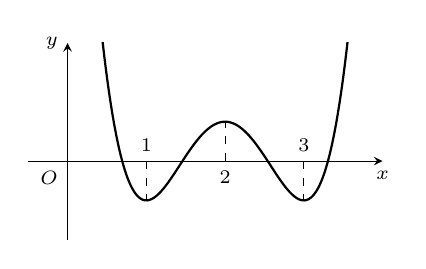
\begin{tikzpicture}[>=stealth,x=1cm,y=1cm,scale=1]
\def\a{1} % Hệ số a phải khác 0
\def\b{-2}
\def\c{.5}
\def\xmin{-.5}
\def\xmax{4}
\def\ymin{-1}
\def\ymax{1.5}
%\draw[color=gray,dash pattern=on 1pt off 1pt,xstep=1.0cm,ystep=1.0cm] (-5.2,-5.2) grid (5.2,5.2);
\draw[->] (\xmin,0) -- (\xmax,0) node[below] {\scriptsize $x$};
\draw[->] (0,\ymin) -- (0,\ymax) node[left] {\scriptsize $y$};
\draw[dashed] (0,0)node[below left]{\scriptsize $O$}
(2,0)node[below]{\scriptsize $2$}--(2,.5) (1,0)node[above]{\scriptsize $1$}--(1,-.5) (3,0)node[above]{\scriptsize $3$}--(3,-.5)
;

\clip (\xmin,\ymin)rectangle(\xmax,\ymax);
\draw[thick,samples=150,smooth,domain=-.5:4] plot(\x,{\a*(\x-2)^4+(\b)*(\x-2)^2+(\c)});
\end{tikzpicture}
\end{center}
Số điểm cực trị của hàm số $y=\left| f(x-1)\right|$ là
\choice
{\True $7$}
{$5$}
{$3$}
{$6$}
\loigiai{
Đồ thị $y=f(x-1)$ là phép tịnh tiến của đồ thị $y=f(x)$ qua bên phải $1$ đơn vị nên số cực trị không thay đổi.\\
Từ đồ thị ta thấy hàm số $y=f(x-1)$ có $2$ điểm cực trị có tung độ âm.\\
Suy ra hàm số $y=\left| f(x-1)\right|$ có $7$ điểm cực trị.
}
\end{ex}

\begin{ex}%[BG12new-4in1, Trần Hoà]%[2D1N1-2]
Cho hàm số $y=f(x)$ có bảng biến thiên như hình bên dưới
\begin{center}

\begin{tikzpicture}[scale=1, line join=round, line cap=round, >=stealth]
\tkzTabInit[nocadre=false,lgt=1.2,espcl=2.5,deltacl=0.6]{$x$/0.6,$y’$ /0.6,$y$ /2}{$-\infty$, $0$,$1$,$+\infty$}
\tkzTabLine{,-,d,-,$0$,+,}
\tkzTabVar{+/$+\infty$,-D+/$-\infty$/$+\infty$,-/$-2$,+/$+\infty$}
\end{tikzpicture}
\end{center}
Khẳng định nào sau đây là \textbf{sai}?
\choice
{Hàm số nghịch biến trên khoảng $(-\infty;-1)$}
{Hàm số nghịch biến trên khoảng $(0;1)$}
{Hàm số đồng biến trên khoảng $(2;+\infty)$}
{\True Hàm số đồng biến trên khoảng $(-2;+\infty)$}
\loigiai{
Từ bảng biến thiên suy ra hàm số đồng biến trên khoảng $(-2;+\infty)$ là sai.
}
\end{ex}
\Closesolutionfile{ans}

\TNTF
\Opensolutionfile{ans}[ans/ansDe1-TN2]
\begin{ex}%giảng 12-4in1, Nhật Thiện]%[2D1V2-7]
\immini{Người ta muốn chế tạo một chiếc hộp hình hộp chữ nhật có thể tích $500\mathrm{cm}^3$. Chiều cao hộp phải là $2$ cm, các kích thước khác là $x, y$ với $x > 0$ và $y > 0$. Gọi $S(x)$ là diện tích toàn phần của chiếc hộp. Xét tính đúng sai các phát biểu sau}{\begin{tikzpicture}[declare function={a=2;b=4;h=2;},line join=round,scale =0.8]
\path (0,0) coordinate (B)
(35:a) coordinate (A)
(b,-1) coordinate (C)
($(C)-(B)+(A)$) coordinate (D)
($(A)+(90:h)$) coordinate (A')
($(B)-(A)+(A')$) coordinate (B')
($(C)-(A)+(A')$) coordinate (C')
($(D)-(A)+(A')$) coordinate (D');
\fill[orange!10] (B)--(B')--(A')--(D')--(D)--(C)--cycle;
\draw ( B')--(B)--(C)--(D)--(D')--(A')--(B')--(C')--(D')  (C)--(C');
\path (B)--(C)node[pos=0.5,sloped,black,below]{$x$};
\path (C)--(D)node[pos=0.5,sloped,black,below]{$y$};
\path (D)--(D')node[pos=0.5,sloped,black,below,scale=0.8]{$2$ cm};
\draw[dashed]  (A')--(A)--(D)  (A)--(B);
\end{tikzpicture}}
\choiceTF[t]
{Khi $x=10$ thì $y=20$}
{\True Diện tích toàn phần của chiếc hộp là $S(x)=500+4 x+\dfrac{1000}{x}$}
{\True Hàm số $S(x)$ nghịch biến trên khoảng $(0;5)$}
{Nếu kích thước của hộp lần lượt là $20$; $12{,}5$; $2$ thì diện tích toàn phần đạt cực tiểu}
\loigiai{
\begin{itemchoice}
\itemch
Ta có $500=x\cdot y \cdot 2 \Rightarrow y=\dfrac{250}{x}$.\\
Với $x=10$ suy ra $y=25$.\\
Phát biểu đã cho sai.
\itemch Diện tích toàn phần của chiếc hộp là
\[S(x)= 2\cdot 2\cdot x+2\cdot 2\cdot y+2\cdot x\cdot y= 500+4 x+\dfrac{1000}{x}.\]
Phát biểu đã cho đúng.
\itemch Lập bảng biến thiên của hàm số $S(x)$ trên khoảng $(0;+\infty)$.\\
Ta có $S'(x)=4-\dfrac{1000}{x^2}$. $S'(x)=0 \Rightarrow x=\pm 5\sqrt{10}$
\begin{center}

\begin{tikzpicture}
\tkzTabInit[nocadre=false,lgt=1.2,espcl=2.5,deltacl=0.6]
{$x$ /0.6,$S'(x)$ /0.6,$S(x)$ /2}
{$0$,$5\sqrt{10}$,$+\infty$}
\tkzTabLine{,-,0,+,}
\tkzTabVar{+/$+\infty$,-/$500+40\sqrt{10}$,+/$+\infty$}
\end{tikzpicture}
\end{center}
Dựa vào bảng biến thiên $S(x)$ nghịch biến trên khoảng $(0;5)$
\itemch
Dựa theo bảng biến thiên ta thấy để diện tích toàn phần đạt cực tiểu thì $x=y=5\sqrt{10}$.\\
Vậy kích thước của hộp là $5\sqrt{10}$; $5\sqrt{10}$; $2$.
\end{itemchoice}
}
\end{ex}

\begin{ex}%[Giải tích $12$ nâng cao, NXBGD Việt Nam, $2020$, Mức độ 3]%[ĐẠI DỰ ÁN TEX HOÁ SGK + GIẢNG LỚP 12]%[12-SCD-CD-2-2 - Thành Đức Trung]
%%[2D1V1-5]
Độ giảm huyết áp của một bệnh nhân được cho bởi công thức $G(x)=0{,}025x^2(30-x)$, trong đó $x$ là liều lượng thuốc được tiêm cho bệnh nhân ($x$ được tính bằng miligam). Mỗi kết quả dưới đây \textbf{đúng} hay \textbf{sai}?
\choiceTF[t]
{\True Khi liều lượng thuốc được tiêm cho bệnh nhân là $30$ mg thì độ giảm huyết áp của bệnh nhân bằng $0$}
{\True Đạo hàm của độ giảm huyết áp theo liều lượng thuốc tiêm cho bệnh nhân là một tam thức bậc hai theo biến $x$}
{Nghiệm của đạo hàm độ giảm huyết áp theo liều lượng là $0$ và $30$}
{Độ giảm huyết áp sẽ giảm khi liều lượng thuốc tăng $0$ đến $20$ mg}
\loigiai
{
\begin{itemchoice}
\itemch Thay $x=30$ vào $G(x)$ ta có $G(30)=0{,}025x^2(30-x)=0$.
\itemch Ta có $G(x)=0{,}025\left(30x^2-x^3\right) \Rightarrow G'(x)=0{,}025\left(60x-3x^2\right) \Rightarrow$ đây là một tam thức bậc hai.
\itemch Xét $G'(x)=0 \Leftrightarrow \hoac{ & x=0 \\ & x=20.}$
\itemch Bảng biến thiên hàm số $G(x)$ trong đoạn $[0;30]$ (vì $G(x)\ge 0$ nên $x\in [0;30]$)
\begin{center}

\begin{tikzpicture}[scale=1]
\tkzTabInit[nocadre=false, lgt=1.2, espcl=3.5, deltacl=0.6]{$x$/0.6, $G'(x)$/0.6, $G(x)$/2}{$0$, $20$, $30$}
\tkzTabLine{0,+,0,-,}
\tkzTabVar{-/$0$, +/$100$, -/$0$}
\end{tikzpicture}
\end{center}
Từ bảng biến thiên ta thấy độ giảm huyết áp sẽ tăng khi liều lượng thuốc tăng $0$ đến $20$ mg.
\end{itemchoice}
}
\end{ex}

\begin{ex}  %[2D1H2-2]
Cho hàm số $ y=\dfrac{-{x^2}-3x+4}{x-3}$ có đồ thị là $( C )$. Những mệnh đề sau \textbf{Đúng} hay \textbf{Sai}?
\choiceTF
{\True Đồ thị $( C )$ có tiệm cận xiên là $ y=-x-6$}
{\True Đồ thị $( C )$ nhận giao điểm $I( 3;-9 )$ làm tâm đối xứng}
{\True Đồ thị $( C )$ có hai điểm cực trị nằm 2 phía đối với $Oy$}
{Đồ thị không cắt trục $Ox$}
\loigiai{
Ta có $ y=-x-6-\dfrac{14}{x-3}$.
\begin{itemchoice}
\itemch Đúng.\\
Đồ thị $( C )$ có tiệm cận xiên là $ y=-x-6$.
\itemch Đúng.\\
Đồ thị $( C )$ nhận giao điểm $I( 3;-9 )$ làm tâm đối xứng.\\
Tiệm cận đứng là $ x=3$.\\
Suy ra, giao điểm 2 tiệm cận là $I( 3;-9 )$ là tâm đối xứng.
\itemch Đúng.\\
Đồ thị $( C )$ có hai điểm cực trị nằm 2 phía đối với $Oy$.\\
Mặt khác, $y'=\dfrac{-x+6x+5}{{{( x-3 )}^2}}=0\Leftrightarrow {x^2}-6x-5=0$. \hfill{$(*)$}\\
Phương trình $(*)$ luôn có 2 nghiệm ${x_1}<0<{x_2}$. \\
Nên $(C)$ luôn có 2 điểm cực trị nằm 2 phía đối với $Oy$.
\itemch Sai.\\
Đồ thị không cắt trục $Ox$.\\
Hơn nữa, $ y=0\Leftrightarrow -{x^2}-3x+4=0$.\\
Phương trình luôn có 2 nghiệm (vì $(-1)\cdot 4<0$).\\
Suy ra $( C )$ cắt $Ox$ tại hai điểm phân biệt.
\end{itemchoice}
}
\end{ex}

\begin{ex}%[TEX NBV, Bồ Văn Hậu]%[2D1H1-3]
Cho hàm số $y=x^3+(m+1) x^2+3x+2$ (tham số $m$).
\choiceTF
{\True Khi $m=-1$ thì hàm số đồng biến trên $(-\infty;+\infty)$}
{\True Đạo hàm của hàm số là $y'=3x^2+2(m+1) x+3$}
{Có $3$ giá trị nguyên dương của tham số $m$ để hàm số $y=x^3+(m+1) x^2+3x+2$ đồng biến trên $\mathbb{R}$}
{Có $6$ giá trị nguyên của tham số $m$ đề hàm số $y=x^3+(m+1) x^2+3x+2$ đồng biến trên $\mathbb{R}$}
\loigiai{
\begin{itemchoice}
\itemch \textbf{Đúng}.\\
Tập xác định $\mathscr{D}=\mathbb{R}$.\\
Khi $m=-1$ ta có $y'=3 x^2+3>0$ nên hàm số đã cho luôn đồng biến trên $(-\infty ;+\infty)$.
\itemch \textbf{Đúng}.\\
Ta có $y'=3 x^2+2(m+1) x+3$.
\itemch \textbf{Sai}.\\
Hàm số $y=x^3+(m+1) x^2+3 x+2$ đồng biến trên $\mathbb{R}$ khi và chỉ khi $y' \geq 0, \forall x \in \mathbb{R}$.
\[\Leftrightarrow \Delta'=(m+1)^2-9 \leq 0 \Leftrightarrow m^2+2 m-8 \leq 0 \Leftrightarrow-4 \leq m \leq 2.\]
Vậy $m \in[-4 ; 2]$ hay có $2$ giá trị nguyên dương của tham số $m$ để hàm số đã cho đồng biến trên $\mathbb{R}$.
\itemch \textbf{Sai}.\\
Vì $m \in[-4 ; 2]$ hay có $7$ giá trị nguyên của tham số $m$ để hàm số đã cho đồng biến trên $\mathbb{R}$.
\end{itemchoice}
}
\end{ex}
\begin{ex}%[2D1H1-2]%[Tổ 1 - Đợt 16 - Chương 1 - Bài 1 - CD]%[Nguyễn Mộng Hùng]
Cho hàm số $f(x)=ax^3+bx^2+cx+d$ $(a \neq 0)$ có bảng biến thiên như sau:
\begin{center}

\begin{tikzpicture}
	\tkzTabInit[nocadre=false,lgt=1.2,espcl=2.5]
	{$x$/.7, $f’(x)$/.7, $f(x)$/2}
	{$-\infty$,$-2$,$1$,$+\infty$}
	\tkzTabLine{ ,-,0,+,0,-, }
	\tkzTabVar{+/$+\infty$,-/$0$,+/$2$,-/$-\infty$}
\end{tikzpicture}
\end{center}
Các mệnh đề sau đúng hay sai?
\choiceTF
{Hàm số $f(x)$ đồng biến trên khoảng $(0; 2)$}
{\True Hàm số $f(x)$ nghịch biến trên khoảng $(2;+\infty)$}
{\True Hàm số $f(x)$ đồng biến trên khoảng $(-2; 1)$}
{\True Hàm số $y=f(2x-1)$ nghịch biến trên khoảng $\left(-\infty;-\dfrac{1}{2}\right)$}
\loigiai
{
\begin{itemchoice}
	\itemch Sai.
	\itemch Đúng.
	\itemch Đúng.
	\itemch Đúng. Xét hàm số $y=f(2x-1)$ có $y'=2f'(2x-1)$.\\
	Hàm số nghịch biến khi $y'\le 0\Leftrightarrow2f'(2x-1)\le 0\Leftrightarrow\hoac{&2x-1\le -2\\&2x-1\ge 1}\Leftrightarrow\hoac{&x\le-\dfrac{1}{2}\\&x\ge 1.}$
	Vậy hàm số $y=f(2x-1)$ nghịch biến trên các khoảng $\left(-\infty;-\dfrac{1}{2}\right)$ và $(1;+\infty)$.
\end{itemchoice}
}
\end{ex}

\begin{ex}%[2D1V2-1]%[Tổ 1 - Đợt 16 - Chương 1 - Bài 1 - CD]%[Nguyễn Mộng Hùng]
Cho hàm số $f(x)=\dfrac{x^2-2x+6}{x+1}$. Các mệnh đề sau đúng hay sai?
\choiceTF
{Hàm số $f(x)$ có tập xác định là $\mathbb{R}$}
{\True Hàm số $f(x)$ có đạo hàm $f'(x)=\dfrac{x^2+2x-8}{(x+1)^2}$}
{Hàm số $f(x)$ có giá trị cực đại bằng $2$}
{\True Hàm số $y=f\left(x^2-2\right)$ có $3$ điểm cực trị}
\loigiai{
\begin{itemchoice}
	\itemch Sai.\\
	Hàm số $f(x)=\dfrac{x^2-2x+6}{x+1}$ xác định khi $x+1\neq 0\Leftrightarrow x \neq-1$.\\
	Do đó, hàm số $f(x)$ có tập xác định là $\mathbb{R}\setminus\{-1\}$.
	\itemch Đúng.
	$$
	f'(x)=\dfrac{\left(x^2-2x+6\right)'(x+1)-\left(x^2-2x+6\right)(x+1)'}{(x+1)^2}=\dfrac{x^2+2 x-8}{(x+1)^2}.
	$$
	\itemch Sai.
	$$
	f'(x)=0 \Leftrightarrow \dfrac{x^2+2 x-8}{(x+1)^2}=0 \Leftrightarrow x^2+2 x-8=0 \Leftrightarrow\hoac{&x=2\\&x=-4.}
	$$
	Bảng biến thiên
	\begin{center}
	
\begin{tikzpicture}
		\tkzTabInit[nocadre=false,lgt=1.2,espcl=2.5]
		{$x$/.7,$f’(x)$/.7,$f(x)$/2}
		{$-\infty$,$-4$,$-1$,$2$,$+\infty$}
		\tkzTabLine{ ,+,0,-,d,-,0,+, }
		\tkzTabVar{-/$-\infty$,+/$-10$,-D+/$-\infty$/$+\infty$,-/$2$,+/$+\infty$}
	\end{tikzpicture}
	\end{center}
	Vậy hàm số $f(x)$ có giá trị cực đại bằng $-10$.
	\itemch Đúng.\\
	Hàm số $y=g(x) = f\left(x^2-2\right)$ xác định khi $x^2-2\neq-1\Leftrightarrow x \neq \pm 1$\\
	$\Rightarrow$ Tập xác định $\mathscr{D}=\mathbb{R}\setminus\{\pm 1\}$.\\
	Có $y'=g'(x)=2x f'\left(x^2-2\right)$.
	$$
	g'(x)=0 \Leftrightarrow\hoac{&2x=0\\&f'(x^2-2)=0}\Leftrightarrow\hoac{&x=0\\&x^2-2=2\\&x^2-2=-4}
	\Leftrightarrow \hoac{&x=0\\&x^2=4\\&x^2=-2}
	\Rightarrow\hoac{&x=0\\&x=2\\&x=-2.}
	$$
	Bảng biến thiên
	\begin{center}
	
\begin{tikzpicture}
		\tkzTabInit[nocadre=false,lgt=1.2,espcl=1.8]
		{$x$/.7,$f’(x)$/.7,$f(x)$/2}
		{$-\infty$,$-2$,$-1$,$0$,$1$,$2$,$+\infty$}
		\tkzTabLine{ ,-,0,+,d,+,0,-,d,-,0,+, }
		\tkzTabVar{+/$+\infty$,-/,+D-/$+\infty$/$-\infty$,+/,-D+/$-\infty$/$+\infty$,-/,+/$+\infty$}
	\end{tikzpicture}
	\end{center}
	Vậy hàm số $y=f\left(x^2-2\right)$ có $3$ điểm cực trị.
\end{itemchoice}
}
\end{ex}

\begin{ex}%[2D1H1-1]%[Tổ 1 - Đợt 16 - Chương 1 - Bài 1 - CD]%[Nguyễn Mộng Hùng]
	Cho hàm số $y=f(x)=\log_5(x^2+4x)$. Các mệnh đề sau đúng hay sai?
	\choiceTF
	{\True Tập xác định của hàm số là $\mathscr{D}=(-\infty;-4) \cup(0;+\infty)$}
	{$f'(x)=\dfrac{2x+4}{\left(x^2+4x\right) \log 5}$}
	{Hàm số $y=f(x)$ nghịch biến trên $(0;+\infty)$}
	{\True Hàm số $y=f(\mathrm{e}^x)$ đồng biến trên $\mathbb{R}$}
	\loigiai{
		\begin{itemchoice}
			\itemch Đúng. Điều kiện $x^2+4x>0\Leftrightarrow\hoac{&x>0\\&x <-4.}$\\
			Tập xác định của hàm số là $\mathscr{D}=(-\infty;-4) \cup(0;+\infty)$.
			\itemch Sai. Ta có $f'(x)=\dfrac{2x+4}{\left(x^2+4x\right)\ln 5}$.
			\itemch Sai. Ta có $f'(x)=0\Rightarrow x=-2$.\\
			Bảng biến thiên
			\begin{center}
				\begin{tikzpicture}
					\tkzTabInit[nocadre=false,lgt=1.2,espcl=3]
					{$x$/.7,$f’(x)$/.7,$f(x)$/2}
					{$-\infty$,$-4$,$0$,$+\infty$}
					\tkzTabLine{ ,-,,h,,+, }
					\tkzTabVar{+/$+\infty$,-H/$-\infty$,-/$-\infty$/,+/$+\infty$}
					\draw (N21)--(N22)(N31)--(N32);
				\end{tikzpicture}
			\end{center}
			Hàm số $y=f(x)$ nghịch biến trên $(-\infty;-4)$.
			\itemch Đúng. Tập xác định $\mathscr{D}=\mathbb{R}$.\\
			Ta có $y'=\left[f(\mathrm{e}^x)\right]'=\mathrm{e}^x\cdot f'(\mathrm{e}^x)=\mathrm{e}^x
			\cdot \dfrac{2\mathrm{e}^x+4}{\left(\mathrm{e}^{2x}+4\mathrm{e}^x\right) \ln 5}>0;\,\forall x\in\mathbb{R}$.\\
			Hàm số $y=f(\mathrm{e}^x)$ đồng biến trên $\mathbb{R}$.
		\end{itemchoice}	
	}
\end{ex}
%%%%==============Cau_EX4==============%%%
\begin{ex}%[2D1H2-1]%[Tổ 1 - Đợt 16 - Chương 1 - Bài 1 - CD]%[Nguyễn Mộng Hùng]
	Cho hàm số $y=f(x)=7^{x^3-x^2-x-1}$. Các mệnh đề sau đúng hay sai?
	\choiceTF
	{\True Tập xác định của hàm số là $\mathscr{D}=\mathbb{R}$}
	{\True $f'(x)=\left(3x^2-2x-1\right)\cdot 7^{x^3-x^2-x-1}\cdot\ln 7$}
	{Hàm số $y=f(x)$ đạt cực đại tại $x=1$}
	{\True Hàm số $y=f(e^x)$ đạt cực tiểu tại $x=0$}
	\loigiai{
		\begin{itemchoice}
			\itemch Đúng. Tập xác định của hàm số là $\mathscr{D}=\mathbb{R}$.
			\itemch Đúng. Ta có $f'(x)=\left(3x^2-2x-1\right) \cdot 7^{x^3-x^2-x-1} \cdot \ln 7$.
			\itemch Sai. Ta có 
			\allowdisplaybreaks
			\begin{eqnarray*}
				&&f'(x)=0\\
				&\Leftrightarrow&\left(3x^2-2x-1\right) \cdot 7^{3^3-x^2-x-1} \cdot \ln 7=0\\
				&\Leftrightarrow& 3x^2-2x-1=0\\
				&\Leftrightarrow&\hoac{&x=1\\&x=-\dfrac{1}{3}\cdot}
			\end{eqnarray*}
			Bảng xét dấu
			\begin{center}
				
\begin{tikzpicture}[font=\normalsize,t style/.style={style=solid}]
					\tkzTabInit[nocadre=false, lgt=1.2, espcl=2.5, deltacl=0.5]
					{$x$/1, $f'(x)$/0.75}
					{$-\infty$, $-\dfrac{1}{3}$, $1$, $+\infty$}
					\tkzTabLine{ , +, 0, -, 0, +}
				\end{tikzpicture}
			\end{center}
			Hàm số đạt cực đại tại $x=-\dfrac{1}{3}$.
			\itemch Đúng. Tập xác định $\mathscr{D}=\mathbb{R}$.\\
			Ta có $y'=\left[f(\mathrm{e}^x)\right]'=\mathrm{e}^x \cdot f'(\mathrm{e}^x)=\mathrm{e}^x \cdot\left(3e^{2x}-2\mathrm{e}^x-1\right) \cdot 7^{\mathrm{e}^{3x}-\mathrm{e}^{2x}-\mathrm{e}^x-1} \cdot \ln 7$.
			$$
			y'=0 \Leftrightarrow 3\mathrm{e}^{2x}-2\mathrm{e}^x-1=0\Leftrightarrow\hoac{&\mathrm{e}^x=1\\&\mathrm{e}^x=-\dfrac{1}{3}}\Rightarrow x=0.
			$$
			Bảng xét dấu
			\begin{center}
				
\begin{tikzpicture}[font=\normalsize,t style/.style={style=solid}]
					\tkzTabInit[nocadre=false, lgt=1.2, espcl=2.5, deltacl=0.5]
					{$x$/0.7, $y'$/0.7}
					{$-\infty$,  $0$, $+\infty$}
					\tkzTabLine{ , -, 0, +, }
				\end{tikzpicture}
			\end{center}
			Hàm số $y=f(\mathrm{e}^x)$ đạt cực tiểu tại $x=0$.
		\end{itemchoice}
	}
\end{ex}
\begin{ex}%[2D1H3-2]%[Tổ 2 - Đợt 16 - Chương 1 - Bài 2 - CD]%[Võ Xuân Cường Thịnh]
	Trong các khẳng định sau, khẳng định nào đúng hay sai?
\choiceTF[t]
{\True	Giá trị nhỏ nhất của hàm số $y=2 x^3+3 x^2-1$ trên đoạn $[-2 ; 1]$ là $-5$}
{		Hàm số $y=4 x^3-12 x^2+9 x$ đạt giá trị lớn nhất trên đoạn $[0 ; 1]$ tại điểm $x=2$}
{Giá trị nhỏ nhất của hàm số $y=\sqrt{4 x-x^2}$ là $4$}
{Hàm số $y=x+\dfrac{4}{x}$ không có giá trị lớn nhất trên khoảng $(0 ;+\infty)$}
\loigiai
{
% Lời giải chung
\begin{itemchoice}
\itemch \textbf{Đúng}. \\
Ta có $y'=6 x^2+6 x$.\\
Trên khoảng $(-2 ; 1), y'=0 \Leftrightarrow \hoac{&x=-1\quad(\text{nhận}) \\ &x=0\quad(\text{nhận}).}$ \\
$y(-2)=-5, y(-1)=0, y(0)=-1, y(1)=4$.\\
Vậy $\min\limits_{[-2;1]} y=y(-2)=-5$.
\itemch \textbf{Sai}. Vì $x=2 \notin \left[0;1\right]$.% Từ lời giải chung đưa ra lí do.
\itemch \textbf{Sai}.  \\% Từ lời giải chung đưa ra lí do.
 Điều kiện $4 x-x^2 \geq 0 \Leftrightarrow 0 \leq x \leq 4$. \\
 Tập xác định của hàm số là $\mathscr{D}=[0 ; 4]$.\\
Ta có $y'=\dfrac{2-x}{\sqrt{4 x-x^2}}$.\\
 Trên khoảng $(0 ; 4)$, ta có $y'=0 \Leftrightarrow 2-x=0 \Leftrightarrow x=2$. \\
 $y(0)=0, y(2)=2, y(4)=0$. \\
 Vậy $\min \limits_{[0;4]} y=y(4)=0$.
\itemch \textbf{Sai}.\\ % Từ lời giải chung đưa ra lí do.
Ta có $y'=1-\dfrac{4}{x^2}=\dfrac{x^2-4}{x^2}$.\\
Trên khoảng $\left(0;+\infty\right)$, ta có $y'=0 \Leftrightarrow x^2-4=0 \Leftrightarrow \hoac{&x=2 \quad(\text{nhận})\\&x=-2. \quad(\text{loại})}$
\begin{center}
	
\begin{tikzpicture}
		\tkzTabInit[nocadre=false,lgt=1.2,espcl=3.5,deltacl=0.6]
		{$x$ /0.6, $y'$ /0.6, $y$ /2.5}
		{$0$,$2$,$+\infty$}
		\tkzTabLine{d,-,$0$,+,}
		\tkzTabVar{+D+/ /+$\infty$,-/$4$,+/$+\infty$}
	\end{tikzpicture}
\end{center}
Dựa vào bảng biến thiên ta thấy không tồn tại giá trị lớn nhất trên $(0;+\infty)$.
\end{itemchoice}
}
\end{ex}
\begin{ex}%[2D1V3-2]%[Tổ 2 - Đợt 16 - Chương 1 - Bài 2 - CD]%[Võ Xuân Cường Thịnh]
	Cho hàm số $y=f(x)$ có đạo hàm như sau 
	$f'(x)=(x-3)(x+3)(x-1)^2$. 
	\choiceTF[t]
	{\True Giá trị lớn nhất của hàm số trên đoạn $[-3 ; 3]$ là $f(-3)$}
	{Hàm số có giá trị lớn nhất trên $\mathbb{R}$}
	{Gọi $g(x)=f(-2 x+3)$. Khi đó giá trị nhỏ nhất của hàm số $g(x)$ trên đoạn $[0 ; 3]$ là $g(3)$}
	{\True Gọi $h(x)=f(-x+5)$ và $h(0)+h(4)=h(2)+h(8)$. \\
		Giá trị lớn nhất của hàm số $h(x)$ trên đoạn $[0 ; 8]$ là $h(8)$}
	\loigiai{
		Ta có BBT
		\begin{center}
			
\begin{tikzpicture}
				\tkzTabInit[nocadre=false,lgt=1.2,espcl=2.5,deltacl=0.6]
				{$x$ /0.6, $y'$ /0.6, $y$ /2.5}
				{$-\infty$,$-3$,$1$,$3$,$+\infty$}
				\tkzTabLine{,+,$0$,-,$0$,-,$0$,+}
				\tkzTabVar{-/$-\infty$,+/$f(3)$,R ,-/$f(3)$,+/$+\infty$}
				%Chen x_0,y_0 vào giữa cột 1 & 2
				\tkzTabIma{2}{4}{3}{$f(1)$}
			\end{tikzpicture}
		\end{center}
		\begin{itemchoice}
			\itemch \textbf{Đúng}.  Dựa vào bảng biến thiên ta có$\min \limits_{[-3 ; 3]} f(x)=f(-3)$.
			\itemch \textbf{Sai}. Dựa vào bảng biến thiên ta thấy hàm số không có giá trị lớn nhất trên $\mathbb{R}$.
			\itemch  \textbf{Sai}.
			Ta có $g^{\prime}(x)=-2 f^{\prime}(-2 x+3)$.
			$$
			\begin{aligned}
				& g^{\prime}(x)=0 \Leftrightarrow-2 f^{\prime}(-2 x+3)=0 \\
				& \Leftrightarrow
				\hoac{
					&- 2 x + 3 = - 3  \\
					& - 2 x + 3 = 1  \\
					& - 2 x + 3 = 3. }
				\Leftrightarrow \hoac{
					&x=3 \\
					&x=1 \\
					&x=0.}	
			\end{aligned}
			$$
					\begin{center}
				
\begin{tikzpicture}
					\tkzTabInit[nocadre=false,lgt=1.2,espcl=2.5,deltacl=0.6]
					{$x$ /0.6, $g'(x)$ /0.6, $g'(x)$ /2.5}
					{$-\infty$,$0$,$1$,$3$,$+\infty$}
					\tkzTabLine{,-,$0$,+,$0$,+,$0$,-}
					\tkzTabVar{+/$+\infty$,-/$g(0)$,R ,+/$g(3)$,-/$-\infty$}
					\tkzTabIma{2}{3}{3}{$g(1)$}
				\end{tikzpicture}
			\end{center}
			Dựa vào bảng biến thiên ta có giá trị nhỏ nhất của hàm số $g(x)$ trên đoạn $[0 ; 3]$ là $g(0)$.
			\itemch \textbf{Đúng}.\\
Ta có $h^\prime(x)=-f(-x+5)$.
\begin{eqnarray*} 
				h^{\prime}(x)=0 &\Leftrightarrow&-f^{\prime}(-x+5)=0 \\
				& \Leftrightarrow&\hoac{
					& - x + 5 = - 3  \\
					&- x + 5 = 1  \\
					& - x + 5 = 3.}\\
		&\Leftrightarrow&\hoac{
					&x=8 \\
					&x=4 \\
					&x=2.}		
\end{eqnarray*}
			\begin{center}
			\begin{tikzpicture}
				\tkzTabInit[nocadre=false,lgt=1.2,espcl=2.5,deltacl=0.5]
				{$x$ /0.6, $h'(x)$ /0.6, $h(x)$ /2.5}
				{$-\infty$,$2$,$4$,$8$,$+\infty$}
				\pattern[pattern=north west lines] (T11) rectangle (N23);
				\pattern[pattern=north west lines] (T21) rectangle (N43);
				\tkzTabLine{,-,$0$,+,$0$,+,$0$,-}
				\tkzTabVar{+/$+\infty$,-/$h(2)$,R ,+/$h(8)$,-/$-\infty$}
				%Chen x_0,y_0 vào giữa cột 1 & 2
				\tkzTabVal{1}{2}{0.5}{$0$}{$h(0)$}
				\tkzTabIma{2}{3}{3}{$h(4)$}
			\end{tikzpicture}
		\end{center}
 Mà \begin{eqnarray*}
 	 h(0)+h(4)&=&h(2)+h(8) \\
				& \Leftrightarrow& h(8)-h(0)=h(4)-h(2) \\
				& \Leftrightarrow& h(8)-h(0)>0(\text { vì } h(4)-h(2)>0) \\
				& \Leftrightarrow& h(8)>h(0).
 \end{eqnarray*}
Vậy giá trị lớn nhất của hàm số trên đoạn $[0 ; 3]$ là $h(8)$.
		\end{itemchoice}
	}
\end{ex}
\begin{ex}%[2D1V3-2]%[Tổ 2 - Đợt 16 - Chương 1 - Bài 2 - CD]%[Võ Xuân Cường Thịnh]
	Cho hàm số $y=f(x)=x^3-3 x^2-9 x+7$. 
	\choiceTF
	{\True Giá trị lớn nhất của hàm số $y=f(x)$ trên đoạn $[-2 ; 0]$ là $12$}
	{Hàm số $y=f(x)+m$ đạt giá trị nhỏ nhất trên đoạn $[-2 ; 0]$ là $10$ khi $m=3$}
	{\True Giá trị nhỏ nhất của hàm số $y=f(2 x^2+1)-5$ là $-25$}
	{Hàm số $y=|f(x)+m|$ đạt giá trị nhỏ nhất trên đoạn $[0 ; 4]$ là $17$ có tích các giá trị của $m$ là $-30$}
	\loigiai{
		\begin{itemchoice}
			\itemch \textbf{Đúng}.\\
Ta có $f^\prime(x)=3x^2-6x-0$.\\
$ f^{\prime}(x)=0 \Leftrightarrow
\hoac{&x=-1 \\
			&x=3.}$\\
Ta có bảng biến thiên
\begin{center}
	\begin{tikzpicture}
		\tkzTabInit[nocadre=false,lgt=1.2,espcl=2.5,deltacl=0.6]
		{$x$ /0.6, $y'$ /0.6, $y$ /2.5}
		{$-\infty$,$-1$,$3$,$+\infty$}
		\pattern[pattern=north west lines] (T11) rectangle (M13);
		\pattern[pattern=north west lines] (T21) rectangle (M23);
		\tkzTabLine{,+,$0$,-,$0$,+,}
		\tkzTabVar{-/$-\infty$,+/$12$,-/$-20$,+/$+\infty$}
		%Chen x_0,y_0 vào giữa cột 1 & 2
		\tkzTabVal{1}{2}{0.5}{$-2$}{$5$}
		\tkzTabVal{2}{3}{0.5}{$0$}{$7$}		
	\end{tikzpicture}
\end{center}
Do đó giá trị lớn nhất của hàm số $y=f(x)$ trên đoạn $[-2 ; 0]$ là 12 .
			\itemch \textbf{Sai}.\\	
	Vì theo câu a ta có bảng biến thiên của hàm số $y=f(x)+m$ là
	\begin{center}
		\begin{tikzpicture}
			\tkzTabInit[nocadre=false,lgt=1.2,espcl=2.5,deltacl=0.6]
			{$x$ /0.6, $y'$ /0.6, $y$ /2.5}
			{$-\infty$,$-1$,$3$,$+\infty$}
			\pattern[pattern=north west lines] (T11) rectangle (M13);
			\pattern[pattern=north west lines] (T21) rectangle (M23);
			\tkzTabLine{,+,$0$,-,$0$,+,}
			\tkzTabVar{-/$-\infty$,+/$12+m$,-/$-20+m$,+/$+\infty$}
			%Chen x_0,y_0 vào giữa cột 1 & 2
			\tkzTabVal{1}{2}{0.5}{$-2$}{$5+m$}
			\tkzTabVal{2}{3}{0.5}{$0$}{$7+m$}		
		\end{tikzpicture}
	\end{center}
	Nên giá trị nhỏ nhất của hàm số $y=f(x)+m$ trên đoạn $[-2 ; 0]$ là $5+m$.\\
	Theo bài ta có $5+m=10 \Leftrightarrow m=5$.
			\itemch \textbf{Đúng}.\\
 Ta có $\left(2 x^2+1\right)^{\prime}=0 \Leftrightarrow x=0$. 
\begin{center}
\begin{tikzpicture}[>=stealth, scale=1]
	\tkzTabInit[lgt=2.4,espcl=2]
	{$x$/1,$2x^+1$/0.8,$f(2x^2+1)$/2}
	{$-\infty$,$-1$,$0$,$1$,$+\infty$}
	\tkzTabLine{+\infty,,3,,1,,3,,+\infty}		
	\tkzTabVar{+/$+\infty$,-/$20$,+D+/$-4$/,-/$-20$,+/$+\infty$}
\end{tikzpicture}
\end{center}
Do đó giá trị nhỏ nhất của hàm số $y=f\left(2 x^2+1\right)-5$ là $-20-5=-25$.
			\itemch \textbf{Sai}.
		\begin{center}
			
\begin{tikzpicture}
				\tkzTabInit[nocadre=false,lgt=2,espcl=2.5,deltacl=1]
				{$x$ /0.6, $f(x)+m$ /2.5}
				{$0$,$3$,$4$}
				\tkzTabVar{+/$7+m$,-/$m-20$,+/$m-13$}
			\end{tikzpicture}
		\end{center}
		Do $7+m>-13+m>-20+m$ nên ta có hai trường hợp
\begin{itemize}
	\item  $\heva{&|7+m|=17 \\ &|7+m|>|-20+m|} \Leftrightarrow \hoac{&m=10\quad(\text{thoả mãn}) \\ &m=-24. \quad(l)}$
\item  $\heva{&|-20+m|=17 \\ 
	&|7+m| \leq|-20+m|} \Leftrightarrow \hoac{&m=3\quad(\text{thoả mãn}) \\ &m=37. \quad(l)}$
\end{itemize}
		\end{itemchoice}
	}
\end{ex}
\begin{ex}%[2D1V3-2]%[Tổ 2 - Đợt 16 - Chương 1 - Bài 2 - CD]%[Võ Xuân Cường Thịnh]
	Cho hàm số $y=f(x)$ liên tục trên đoạn $\mathbb{R}$ và có đồ thị như hình vẽ.
	\begin{center}
		
\begin{tikzpicture}
			\tkzTabInit[nocadre,lgt=1.2,espcl=2.5,deltacl=0.6]
			{$x$ /0.6,$y'$ /0.6,$y$ /2}
			{$-\infty$,$-2$,$0$,$2$,$+\infty$}
			\tkzTabLine{,+,$0$,-,$0$,+,$0$,-,}
			\tkzTabVar{-/$-\infty$, +/$4$,-/$0$,+/$4$,-/$-\infty$}
		\end{tikzpicture}
	\end{center}
Khi đó
	\choiceTF[t]
	{\True $\max\limits_{[0 ; 2]} f(x)=4$}
	{ Hàm số $y=f(x)$ có giá trị lớn nhất là $4$ và giá trị nhỏ nhất là $0$}
	{Hàm số $y=f(2 \cos x)$ có giá trị lớn nhất là 4 tại $x=\dfrac{\pi}{2}$}
	{Không tồn tại giá trị lớn nhất của hàm số $y=f(f(x))$ trên $(-2 ; 2)$}
	\loigiai{
		\begin{itemchoice}
			\itemch \textbf{Đúng}. Dựa vào bảng biến thiên ta có $\max\limits_{[0 ; 2]} f(x)=4$ tại $x=2$.
			\itemch \textbf{Sai}.Dựa vào bảng biến thiên hàm số không có giá trị nhỏ nhất.
			\itemch  \textbf{Sai}.\\
			Đặt $t=2 \cos x, t \in[-2 ; 2]$, ta có $y=f(2 \cos x)=f(t)$.\\
			$\max \limits_{\mathbb{R}} f(2 \cos x)=\max\limits_{[-2 ; 2]} f(t)=4$ khi $t= \pm 2$, tức là $\cos x= \pm 1$. \\
			Mà $\cos \dfrac{\pi}{2}=0$ nên hàm số $y=f(2 \cos x)$ không đạt giá trị lớn nhất tại $x=\dfrac{\pi}{2}$.
			\itemch \textbf{Sai}.\\
			Đặt $t=f(x)$, ta có $y=f(f(x))=f(t), x \in (-2;2) \Rightarrow t \in [0;4)$.\\
			Ta có $\max\limits_{[-2 ; 2]}f(f(x))=\max\limits_{[0;4)}f(t)=4$ khi $t=2$.
		\end{itemchoice}
	}
\end{ex}
\Closesolutionfile{ans}

\TNSA
\Opensolutionfile{ans}[ans/ansDe1-TN3]
\begin{ex}%[2D1C1-2]%[Tổ Latex - Strong]%[Tổ 1 - Đợt 16 - Chương 1- Bài 1 - CD]%[DuongPham]
	\immini{	Cho hàm số $f(x)$ có đạo hàm liên tục và xác định trên $\mathbb{R}$ và có đồ thị hàm số $f'(x)$ như hình vẽ bên.
		Biết hàm số $g(x)=f\left(x^2-2 x\right)$  đồng biến trên $(-\infty ; a)$ và $(b ; c)$ và nghịch biến trên $(a;b)$ và $(c ; +\infty)$ . Tính $a+b+c$.}{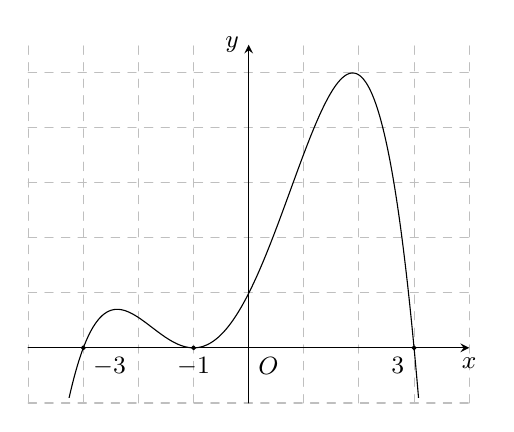
\begin{tikzpicture}[scale=0.7,>=stealth, font=\small, line join=round, line cap=round]
			\def\a{-0.11} \def\b{-4} \def\c{3} % Hệ số
			\def\xmin{-4} \def\xmax{4}
			\def\ymin{-1} \def\ymax{5.5}
			
			\draw[color=gray!50,dashed] (\xmin,\ymin) grid (\xmax,\ymax);
			
			\draw[->] (\xmin,0)--(\xmax,0) node [below]{$x$};
			\draw[->] (0,\ymin)--(0,\ymax) node [left]{$y$};
			\node at (0,0) [below right]{$O$};
			\clip (\xmin+0.1,\ymin+0.1) rectangle (\xmax-0.5,\ymax-0.1);
			\draw[smooth,samples=300] plot(\x,{\a*(\x+1)^2*(\x+3)*(\x-3)});
			\draw[fill=black](-3,0)node[below right]{$-3$}circle(1pt)
			(-1,0)node[below]{$-1$}circle(1pt)
			(3,0)node[below left]{$3$}circle(1pt)
			;
	\end{tikzpicture}}
	\shortans{$3$}
	\loigiai
	{		Xét hàm số $g(x)=f\left(x^2-2 x\right)$ có $g'(x)=(2 x-2) \cdot f'\left(x^2-2 x\right)$.
		$$
		g'(x)=0 \Leftrightarrow\hoac{&
			2 x - 2 = 0  \\
			& f ' ( x^2 - 2 x ) = 0 
		} \Leftrightarrow \hoac{
			& 2 x - 2 = 0  \\
			& x^2 - 2 x = - 3  \\
			& x^2 - 2 x = - 1  \\
			& x^2 - 2 x = 3 
		} \Leftrightarrow \hoac{
			&x=1 \\
			&x=-1 \\
			&x=3.}$$
		Ta có bảng sau
		\begin{center}
			
\begin{tikzpicture}
				\tkzTabInit[nocadre=false,lgt=2,espcl=2,deltacl=0.6]
				{$x$ /0.6,$g'(x)$ /0.6}
				{$-\infty$,$-1$,$1$,$3$,$+\infty$}
				\tkzTabLine{,+,$0$,-,$0$,+,$0$,-,}
			\end{tikzpicture}
		\end{center}	
		Do đó, hàm số $g(x)=f\left(x^2-2 x\right)$ đồng biến trên các khoảng $(-\infty ;-1)$ và $(1 ; 3)$.
		Suy ra $a=-1, b=1, c=3$. Vậy $a+b+c=3$.
	}
\end{ex}
\begin{ex}%[2D1V1-2]%[Tổ Latex - Strong]%[Tổ 1 - Đợt 16 - Chương 1- Bài 1 - CD]%[DuongPham]
	Biết hàm số $y =-x^4 +2x^2 +1$ đồng biến trên $(-\infty ; a)$ và $(b ; c)$ và nghịch biến trên $(a;b)$ và $(c;+\infty)$. Tính $a+2024b+c$.
	\shortans{$0$}
	\loigiai{Tập xác định $\mathscr{D}=\mathbb{R}$.\\ Ta có $y'=-4x^3+4x$, $y'=0\Leftrightarrow \hoac{&x=0\\&x=\pm1.}$\\
		Bảng biến thiên
		\begin{center}
			
\begin{tikzpicture}
				\tkzTabInit[nocadre=false,lgt=1.2,espcl=2.5,deltacl=0.6]
				{$x$ /0.6,$y'$ /0.6,$y$ /2}
				{$-\infty$,$-1$,$0$,$1$,$+\infty$}
				\tkzTabLine{,+,$0$,-,$0$,+,$0$,-,}
				\tkzTabVar{-/$-\infty$, +/$2$,-/$1$,+/$2$,-/$-\infty$}
			\end{tikzpicture}
		\end{center}
		Từ bảng biến thiên ta thấy tất cả các khoảng nghịch biến của hàm số là $(-1;0)$ và $(1;+\infty)$. Suy ra $a = -1$, $b = 0$, $c = 1$. Vậy $a + 2024b + c = 0$.
	}
\end{ex}
\begin{ex}%[2D1V1-3]%[Tổ Latex - Strong]%[Tổ 1 - Đợt 16 - Chương 1- Bài 1 - CD]%[DuongPham]
	Cho hàm số $y = \dfrac{x^2 +x+m^2 -6}{x + 2}$. Tìm số giá trị nguyên của tham số $m$ để hàm số đơn điệu trên mỗi khoảng xác định.
	\shortans{$5$}
	\loigiai{
		Tập xác định $\mathscr{D}=\mathbb{R}$.\\
		Ta có $y'= \dfrac{x^2+4x-m^2+8}{(x+2)^2}$.\\
		Hàm số đơn điệu trên mỗi khoảng xác định khi và chỉ khi đạo hàm $y'$ không đổi dấu trên mỗi khoảng xác định.
		\begin{itemize}
			\item[TH1.] Phương trình $x^2 + 4x - m^2 + 8 = 0$ có nghiệm kép khi và chỉ khi $(x + 2)^2 = m^2 - 4$ có nghiệm kép khi và chỉ khi $m=\pm2$.
			\item[TH2.] $x^2 + 4x - m^2 + 8 = 0$ vô nghiệm khi và chỉ khi $(x + 2)^2 = m^2 -4$ vô nghiệm khi và chỉ khi $m^2 -4<0\Leftrightarrow -2<m<2$.
		\end{itemize}
		Vậy có 5 giá trị nguyên của tham số $m$ để hàm số đơn điệu trên mỗi khoảng xác định.		
	}
\end{ex}
\begin{ex}%[2D1V1-5]%[Tổ Latex - Strong]%[Tổ 1 - Đợt 16 - Chương 1- Bài 1 - CD]%[DuongPham]
	Thể tích $V$ của $1$ kg nước ở nhiệt độ $T$ ($0^\circ\le T\le30^\circ$) được cho bởi công thức  $V =999{,}87-0{,}06426T+0{,}0085043T^2 -0{,}0000679T^3$ (Theo: J. Stewart, Calculus, Seventh
	Edition, Brooks/Cole, CENGAGE Learning 2012). Gọi $(a^\circ ;b^\circ)$
	là khoảng nhiệt độ lớn nhất mà trong
	khoảng đó khi nhiệt độ tăng thì thể tích $V$ của $1$kg nước cũng tăng. Tính giá trị biểu thức $P = b - a$
	($a$, $b$ làm tròn đến hàng đơn vị).
	\shortans{$26$}
	\loigiai{
		Xét hàm số $f (T)=999{,}87-0{,}06426T+0{,}0085043T^2 -0{,}0000679T^3$ với $0^\circ \le T \le30^\circ$.\\
		Nhiệt độ tăng thì thể tích của 1kg nước tăng tức hàm số $f (T )$ đồng biến.\\
		$f'(T)=-0{,}06426+0{,}0170086T -2{,}037\cdot10^{-4}T^2$.\\
		$f'(T)=0\Leftrightarrow\hoac{& T_1 \approx 3{,}966\in[0;30]\\
			&T_2 \approx 79{,}532\notin[0;30].}$\\
		$f '(T )> 0,\forall T \in(T_1 ;T_2 )$ nên hàm số $f (T)$ đồng biến trên khoảng $(T_1 ;T_2 )$.\\
		Suy ra khi $T\in(T_1^\circ ;30^\circ)$ 1
		thì khi nhiệt độ nước tăng thể tích của 1kg nước cũng tăng.\\
		Suy ra $a=4$, $b=30$. Vậy $b-a=26$.
	}
\end{ex}
\begin{ex}%[2D1V1-2]%[Tổ Latex - Strong]%[Tổ 1 - Đợt 16 - Chương 1- Bài 1 - CD]%[DuongPham]
	Trên khoảng $(0;100)$ hàm số $y=2 \sin ^2 x-x$ có bao nhiêu điểm cực đại?
	\shortans{$32$}
	\loigiai{	Tập xác định $\mathscr{D}=\mathbb{R}$.\\
		Ta có $y'=4 \sin x \cos x-1=2 \sin 2 x-1$.
		$$
		y'=0 \Leftrightarrow \sin 2 x=\dfrac{1}{2} \Leftrightarrow\hoac{
			& 2 x = \dfrac { \pi } { 6 } + k 2 \pi  \\
			& 2 x = \dfrac { 5 \pi } { 6 } + k 2 \pi 
		} \Leftrightarrow\hoac{
			&x=\dfrac{\pi}{12}+k \pi \\
			&x=\dfrac{5 \pi}{12}+k \pi
		} \quad(k \in \mathbb{Z}).
		$$
		\begin{itemize}
			\item Với $x=\dfrac{\pi}{12}+k \pi$.\\
			Do $x \in(0 ; 100)$ nên $0<\dfrac{\pi}{12}+k \pi<100 \Leftrightarrow-\dfrac{1}{12}<k<\dfrac{100}{\pi}-\dfrac{1}{12} \Rightarrow k \in\{0 ; 1 ; \ldots ; 31\}$.
			\item Với $x=\dfrac{5 \pi}{12}+k \pi$.\\
			Do $x \in(0 ; 100)$ nên $0<\dfrac{5 \pi}{12}+k \pi<100 \Leftrightarrow-\dfrac{5}{12}<k<\dfrac{100}{\pi}-\dfrac{5}{12} \Rightarrow k \in\{0 ; 1 ; \ldots ; 31\}$.
		\end{itemize}
		Như vậy phương trình $y'=0$ có $64$ nghiệm trên khoảng $(0 ; 100)$ đồng thời $y'$ đổi dấu qua $64$ nghiệm đó. Vậy số điểm cực đại của hàm số đã cho là $32$.		
	}
\end{ex}
\begin{ex}%[2D1V1-5]%[Tổ Latex - Strong]%[Tổ 1 - Đợt 16 - Chương 1- Bài 1 - CD]%[DuongPham]
	\immini{Một công ty muốn xây dựng hệ thống dây cáp từ trạm A ở trên bờ biển đến một vị trí B trên một hòn đảo. Hòn đảo cách bờ biển 6 km . Gọi C là điểm trên bờ sao cho BC vuông góc với bờ biển. Khoảng cách từ A đến C là $9$ km . Giá để lắp đặt mỗi km hệ thống dây trên bờ là $50$ triệu đồng và dưới nước là $130$ triệu đồng. Người ta cần xác định một vị trí D trên AC để lắp đặt hệ thống dây theo đường gấp khúc ADB mà số tiền chi phí thấp nhất. Khi đó chi phí lắp đặt thấp nhất là bao nhiêu triệu đồng?}{\begin{tikzpicture}[>=stealth,line join=round,line cap=round,font=\small,scale=1]
			\path
			(0,0)coordinate(C)
			(0,3.5)coordinate(B)
			(2,0)coordinate(D)
			(4,0)coordinate(A)
			;
			\draw(B)--(C)--(A)
			(B)--(D);
			\draw($(B)!0.5!(C)$)node[left]{$6$km}
			($(A)!0.5!(C)$)node[below]{$9$km}
			;
			\foreach \x/\g in {C/180,A/90,D/60,B/180}\fill[black](\x)circle(1pt)+(\g:.3)node{$\x$};
	\end{tikzpicture}}
	\shortans{$1170$}
	\loigiai{Đặt $C D=x(\mathrm{km})\,(x \in[0 ; 9])$.\\
		Ta có $A D=9-x(\mathrm{km})$ và $B D=\sqrt{C D^2+B C^2}=\sqrt{x^2+36}(\mathrm{km})$.\\
		Chi phí lắp đặt là $F(x)=50(9-x)+130 \sqrt{x^2+36}$ (triệu đồng).\\
		Xét hàm số $F(x)=50(9-x)+130 \sqrt{x^2+36}$ trên $[0 ; 9]$.\\
		$F'(x)=-50+\dfrac{130 x}{\sqrt{x^2+36}}$. \allowdisplaybreaks
		\begin{eqnarray*}
			F'(x)=0 &\Leftrightarrow& \dfrac{130 x}{\sqrt{x^2+36}}-50=0\\
			& \Leftrightarrow& 13 x=5 \sqrt{x^2+36} \Leftrightarrow\heva{&
				x \geq 0 \\
				&169 x^2=25\left(x^2+36\right)}\\
			& \Leftrightarrow& x=\dfrac{5}{2}(\text{thỏa mãn}).
		\end{eqnarray*}
		Bảng biến thiên
		\begin{center}
			
\begin{tikzpicture}
				\tkzTabInit[nocadre=false,lgt=1.2,espcl=2.5,deltacl=0.6]
				{$x$ /0.6,$F'(x)$ /0.6,$F(x)$ /2}
				{$0$,$\tfrac52$,$9$}
				\tkzTabLine{,-,$0$,+,}
				\tkzTabVar{+/$1230$, -/$1170$,+/$390\sqrt{13}$}
			\end{tikzpicture}
		\end{center}
		Vậy chi phí thấp nhất để lắp đặt hệ thống dây cáp là $1170$ triệu đồng.
	}
\end{ex}
\begin{ex}%[Đỗ Minh Phúc]%[2D1V1-3]
Có bao nhiêu giá trị nguyên $m$ thuộc $[-7;7]$ để hàm số $y=\dfrac{mx+1}{x+m}$ đồng biến trên khoảng $(1; 5)$.
\shortans[]{$9$}
\loigiai{
Tập xác định $\mathscr{D}=\mathbb{R}\backslash \{-m\}$. Đạo hàm $y'=\dfrac{m^2-1}{(x+m)^2}$. \\
Hàm số đồng biến trên khoảng $(1; 5)$ khi và chỉ khi
\[\heva{&-m\notin (1; 5) \\ &m^2-1>0} \Leftrightarrow \heva{&m\in (-\infty; 1]\cup [5; +\infty) \\ &m\in (-\infty; -1)\cup (1; +\infty)} \Leftrightarrow m\in (-\infty; -1)\cup [5; +\infty).\]
Có $9$ giá trị nguyên của $m$ là $m=\{-7;-6;-5;-4;-3;-2;5;6;7\}$.
}
\end{ex}

\begin{ex}%[2D1H1-2]
Hàm số $ y=| {x^2}+5x+6 |$ có mấy điểm cực trị?
\shortans{$3$}
\loigiai{$y=\left|x^2+5x+6\right|=\sqrt {{{\left(x^2+5x+6\right)}^2}}$\\
Hàm số đã cho xác định trên $D=\mathbb{R}$.\\
\[y'=\dfrac{\left(2x+5\right)\left(x^2+5x+6\right)}{\sqrt {{{\left(x^2+5x+6\right)}^2}}}\, \forall x\in \mathbb{R}\setminus \{-2;-3\}\]
Hàm số không có đạo hàm tại $x=0$ và $x=2$.\\
Cho $y'=0\Leftrightarrow (2x+5)(x^2+5x+6)=0\Leftrightarrow \hoac{& 2x+5=0\\
& x^2+5x+6=0}\Leftrightarrow \hoac{& x=-\dfrac{5}{2} \\
& x=-2\\
& x=-3}$ \\
Dựa vào bảng biến thiên:\\
Hàm số có 2 cực tiểu $( -3{,}0 );( -2{,}0 )$; Hàm số có 1 cực đại $\left( -\dfrac{5}{2},-\dfrac{1}{4} \right) $.
}
\end{ex}

\begin{ex}%[MĐ3]%[2D1V2-6]
Giả sử $a$, $b$ là các số thực sao cho đồ thị hàm số $y=\dfrac{2x^2-ax+5}{x^2+b}$  có điểm cực đại là $\left(\dfrac{1}{2};6\right)$, tính giá trị của $ab$. \shortans{$-4$}
\loigiai{
Ta có $y'=\dfrac{ax^2+2(2b-5)x-ab}{\left(x^2+b\right)^2}$. Đồ thị hàm số có điểm cực đại là $\left(\dfrac{1}{2};6\right)$  nên
\begin{align*}
\heva{&y'\left(\frac{1}{2}\right)=0\\ &y\left(\frac{1}{2}\right)=6} \Rightarrow \heva{&\frac{1}{4}a+2b-5-ab=0\\ & \frac{\dfrac{1}{2}-\dfrac{a}{2}+5}{b+\dfrac{1}{4}}=6\\ &b\ne -\frac{1}{4}.}
\end{align*}
Từ phương trình thứ hai, ta có $a=8-12b$, thay vào phương trình thứ nhất, ta được
\[ 12b^2-9b-3=0 \Leftrightarrow \hoac{&b=1\\ &b=-\dfrac{1}{4}.} \]
Kết hợp với điều kiện $b\ne -\dfrac{1}{4}$, ta được $b=1$, suy ra $a=-4$.

Khi đó $y'=\dfrac{-4x^2-6x+4}{\left(x^2+1\right)^2}$, $y'=0 \Leftrightarrow x=-2$ hoặc $x=\dfrac{1}{2}$. Ta có bảng biến thiên
\begin{center}

\begin{tikzpicture}[font=\small,>=stealth, scale=1]
\tkzTabInit[nocadre=false,lgt=1.2,espcl=2.5,deltacl=0.6]
{$x$ /1,$y'$ /0.6,$y$ /2}
{$-\infty$, $-2$, $\dfrac{1}{2}$, $+\infty$}
\tkzTabLine{,-,0,+,0,-,}
\tkzTabVar{+/$2$, -/$1$, +/$6$, -/$2$}
\end{tikzpicture}
\end{center}
Vậy $(a,b)=(-4,1)$ và $ab=-4$.
}
\end{ex}

\begin{ex}%[De-chuan-hoa-so-13]%[Lê Toàn]%[2D1H1-3]
Số giá trị nguyên của tham số $m$ để hàm số $y=\dfrac{x+2}{x+3m}$ đồng biến trên khoảng $(-\infty;-6)$ là
\shortans{$2$}
\loigiai{
Điều kiện xác định $x \neq -3m$.\\
Ta có $y'=\dfrac{3m-2}{(x+3m)^2}$.\\
Để hàm số đồng biến trên khoảng $(-\infty;-6)$ khi và chỉ khi $y'>0$, $\forall x \in (-\infty;-6)$.\\
Khi đó, $\heva{&-3m \notin (-\infty;-6)\\&3m-2>0} \Leftrightarrow \heva{&-3m \geq -6 \\&3m-2>0} \Leftrightarrow \heva{&m \leq 2 \\&m>\dfrac{2}{3}} \Leftrightarrow \dfrac{2}{3}<m \leq 2$.\\
Với $m \in \mathbb{Z}$ nên $m\in \{1;2\}$. Vậy có $2$ giá trị thỏa mãn yêu cầu bài toán.
}
\end{ex}

\begin{ex}%[2D1H2-4]
Tìm tổng các giá trị nguyên dương của tham số $m$ để hàm số $y=x^3+(m-1)x^2+3x-2$ không có cực trị.
\shortans[]{$7$}
\loigiai{
Hàm số không có cực trị $\Leftrightarrow y'=3x^2+2(m-1)x+3=0$ vô nghiệm hoặc có nghiệm kép $\Leftrightarrow \Delta'=(m-1)^2-9 \leq 0 \Leftrightarrow m^2-2m-8 \leq 0 \Leftrightarrow-2\leq m \leq 4$.\\
Suy ra tổng các giá trị nguyên là $7$.}
\end{ex}

\begin{ex}%[2D1H2-6]
Cho hàm số $y=\dfrac{x^2+(m+1)x+2m+1}{x+1}$. Số nguyên bé nhất $m$ để hàm số sau đây có 2 điểm cực trị.
\shortans[]{$0$}
\loigiai{Tập xác định $\mathscr{D}=\mathbb{R}\setminus \{-1\}$.\\
Ta có $y'=\dfrac{x^2+2x-m}{(x+1)^2}$.\\
Để hàm số có hai điểm cực trị thì phương trình $x^2+2x-m=0$ có hai nghiệm đơn phân biệt $x_1$, $x_2$ khác $-1$. Điều này tương đương $\heva{&1+m>0\\&-1-m\neq 0}\Leftrightarrow m>-1$.
Suy ra số nguyên bé nhất là $0$.
}
\end{ex}
\begin{ex}%[2D1N3-1]%[Tổ 2-Đợt 16-Chương 1-Bài 2-Cánh Diều]%[Loc Do]
	Tìm giá trị nhỏ nhất của hàm số $y=x^3-3x+4$ trên đoạn $\left[0;2\right]$.
	\shortans{$2$}
	\loigiai{Tập xác định $\mathscr{D}=\mathbb{R}$.
		\[y'=3x^2-3; \,y'=0\Leftrightarrow 3x^2-3=0\Leftrightarrow \hoac{&{x=1\in \left[0;2\right]} \\
			&{x=-1\notin \left[0;2\right] (\text{loại}).}}
		\]
		Ta có $f(0)=4$, $f(2)=6$, $f(1)=2$.
		Do đó $\min\limits_{\left[0;2\right]} y=2$.
	}
\end{ex}
%%%==============BT_2==============%%%
\begin{ex}%[2D1N3-1]%[Tổ 2-Đợt 16-Chương 1-Bài 2-Cánh Diều]%[Loc Do]
	Cho hàm số $y=f(x)$ liên tục và có bảng biến thiên trên đoạn $\left[-1; 3\right]$ như hình vẽ bên. Giả sử giá trị lớn nhất của $y=f(x)$ trên $\left[-1; 3\right]$ đạt được tại giá trị $x_0$. Tìm $x_0$
	\begin{center}
		
\begin{tikzpicture}[>=stealth]
			\tkzTabInit[nocadre=false,lgt=1,espcl=2,deltacl=0.5]{$x$/.7 ,$y'$/.7,$y$/2}
			{$-1$ , $0$ , $2$ , $3$}
			\tkzTabLine{ , + , $0$ , - , $0$ , + , }
			\tkzTabVar{-/$0$ , +/$5$ , -/$1$ , +/$4$}
		\end{tikzpicture}		
	\end{center}
	\shortans{$0$}
	\loigiai{
		Nhìn vào bảng biến thiên ta thấy $\max\limits_{\left[-1;3\right]} f(x)=5=f(0)$. \\
		Vậy giá trị lớn nhất của $y=f(x)$ trên $\left[-1; 3\right]$ đạt được tại $x_0=0$.
	}
\end{ex}
%%%==============BT_3==============%%%
\begin{ex}%[2D1V3-1]%[Tổ 2-Đợt 16-Chương 1-Bài 2-Cánh Diều]%[Loc Do]
	\immini{Cho hàm số có $f(x)$ có đạo hàm là hàm $f'(x)$. Đồ thị hàm số $f'(x)$ như hình vẽ bên. Biết rằng $f(0)-f(2)=f(4)-f(3)$. Giả sử giá trị nhỏ nhất $m$ và giá trị lớn nhất $M$ của $f(x)$ trên đoạn $\left[0;4\right]$ đạt được lần lượt tại $x_0$ và $x_1$. Tổng $x_0$ và $x_1$ là}{
		\begin{tikzpicture}[x=.5cm,y=.5cm,scale=1]
			\draw[->] (-1,0)--(8,0)node[below right]{$x$};
			\draw[->] (0,-3)--(0,4)node[left]{$y$};
			\draw (0,0) circle (0.5pt)  node[below left]{ $O$};
			\draw[blue] (-0.25,-1.54)..controls (0,0) and (0.42,2.18)..(0.55,2.34) ;
			\draw[blue] (0.55,2.34)..controls (1.3,3.74) and (1.7,0.48)..(2.74,-2.05) ;
			\draw[blue] (2.74,-2.05)..controls (3.48,-3.26) and (5.16,-2.12)..(7.66,-0.56) ;
			\foreach \x/\g in {2/-120,4/-90}
			\draw[thin] (\x,2pt)--(\x,-2pt) + (\g:3mm) node {$\x$};
		\end{tikzpicture}
	}
	\shortans{$6$}
	\loigiai{
		Dựa vào đồ thị của hàm $f'(x)$ ta có bảng biến thiên.
	\begin{center}
		
\begin{tikzpicture}[>=stealth]
			\tkzTabInit[nocadre=false,lgt=2,espcl=2,deltacl=0.5]{$x$/.7 ,$f'(x)$/.7,$f(x)$/2}
			{$0$ , $2$ , $4$}
			\tkzTabLine{ , + , $0$ , - , }
			\tkzTabVar{-/$f(0)$ , +/$f(2)$ , -/$f(4)$}
		\end{tikzpicture}
	\end{center}
		Vậy giá trị lớn nhất $M=f(2)\Rightarrow x_1=2$.\\
		Hàm số nghịch biến trên khoảng $\left(2;4\right)$ nên $f(2) > f(3)\Rightarrow f(2)-f(3) > 0$.\\
		Ta có 
		\begin{eqnarray*}
			&& f(0)-f(2)=f(4)-f(3)\\
			&\Leftrightarrow& f(0)-f(4)=f(2)-f(3) > 0\\
			&\Rightarrow& f(0) > f(4)
		\end{eqnarray*}
		Suy ra giá trị nhỏ nhất $m=f(4)\Rightarrow x_0=4$.
		Vậy $x_0=4; x_1=2$, ta có $x_0+x_1=6$.
	}
\end{ex}
%%%==============BT_4==============%%%
\begin{ex}%[2D1H4-3]%[Tổ 2-Đợt 16-Chương 1-Bài 2-Cánh Diều]%[Loc Do]
	Gọi $S$ là tập hợp chứa các tham số $m$ để đồ thị hàm số $y=\dfrac{mx-1}{x+m}$ có tiệm cận đứng và tiệm cận ngang tạo với các trục tọa độ hình chữ nhật có diện tích bằng $4$. Số phần tử của $S$ là
	\shortans{$2$}
	\loigiai{
		Phương trình tiệm cận ngang là $y=m$.\\
		Phương trình tiệm cận đứng là $x=-m$.\\
		Theo đề bài ta có $\left|m\right|\cdot\left|-m\right|=4\Leftrightarrow m^2=4\Leftrightarrow m=\pm 2$.
		Vậy $S$ có $2$ phần tử.
	}
\end{ex}
%%%==============BT_5==============%%%
\begin{ex}%[2D1V3-6]%[Tổ 2-Đợt 16-Chương 1-Bài 2-Cánh Diều]%[Loc Do]
	Giả sử số lượng của một quần thể nấm men tại môi trường nuôi cấy trong phòng thí nghiệm được mô hinh hoá bằng hàm số $P(t)=\dfrac{a}{b+\mathrm{e}^{-0,75t}}$, trong đó thời gian $t$ được tính bằng giờ. Tại thời điểm ban đầu $t=0$, quần thể có 20 tế bào và tăng với tốc độ 12 tế bào/giờ. Tìm các giá trị của $a$ và $b$. Theo mô hình này, số lượng nấm men không vượt quá bao nhiêu?
	\shortans{$100$}
	\loigiai{
		Ta có $P'(t)=\dfrac{0,75a \mathrm{e}^{-0{,}75t}}{\left(b+\mathrm{e}^{-0{,}75t} \right)^2},\,\, t\ge 0$.\\
		Theo đề bài, ta có $P(0)=20$ và $P'(0)=12$. \\
		Do đó, ta có hệ phương trình $\heva{&{\dfrac{a}{b+1}=20} \\
			&{\dfrac{0,75a}{(b+1)^2}=12}}\Leftrightarrow \heva{&{a=20(b+1)} \\
			&{\dfrac{15}{b+1}=12.}}$\\
		Giải hệ phương trình này, ta được $a=25$ và $b=\dfrac{1}{4}$.\\
		Khi đó, $P'(t)=\dfrac{18,75\mathrm{e}^{-0,75t}}{\left(\tfrac{1}{4}+\mathrm{e}^{-0,75t} \right)^2} > 0,\forall t\ge 0$, tức là số lượng quần thể nấm men luôn tăng.\\
		Tuy nhiên, do $\lim\limits_{t\to+\infty} P(t)=\lim\limits_{t\to+\infty} \dfrac{25}{\tfrac{1}{4}+\mathrm{e}^{-0.75t}}=100$ nên số lượng quần thể nấm men tăng nhưng không vượt quá $100$ tế bào.
	}
\end{ex}
%%%==============BT_6==============%%%
\begin{ex}%[2D1C3-4]%[Tổ 2-Đợt 16-Chương 1-Bài 2-Cánh Diều]%[Loc Do]
\immini{Cho hàm số $y=f(x)$ là hàm đa thức bậc hai và có đồ thị hàm số $f\left(x^2-1\right)$ như hình vẽ.	Đặt $g(x)=\left|f(x^2)+m\right|$. Có bao nhiêu giá trị nguyên thuộc $[-2024;2024]$ của tham số $m$ để với mọi bộ ba số phân biệt $a,b,c$ thuộc $[-2;2]$ ta đều có bộ ba số $g(a);g(b);g(c)$ là số đo độ dài ba cạnh của một tam giác? }{\begin{tikzpicture}[scale=1,>=stealth]
		\def\aa{-1} \def\bb{4} \def\cc{0}
		\draw[color=gray,dash pattern=on 1pt off 1pt,xstep=1.0cm,ystep=1.0cm] (-2.5,-1.5) grid (2.5,4.5);
		\draw[->] (-2.21,0)--(2.21,0)node[below right]{$x$};
		\draw[->] (0,-1.01)--(0,5)node[left]{$y$};
		\fill (0,0)node[below left]{$O$};
		\draw[black,samples=150,smooth,domain=-2.05:2.05] plot(\x,{\aa*(\x)^4+\bb*(\x)^2+\cc});
		\end{tikzpicture}}
\shortans{$4021$}
	\loigiai{
		Từ đồ thị ta có $f\left(x^2-1\right)=k x^2(x^2-4)=h(x)$.\\
		Vì $h'(x)=k\left(4x^3-8x\right)=0\Leftrightarrow \hoac{&x=0\\ &x=\pm \sqrt{2}.}$\\
		Dựa theo đồ thị $h\left(\sqrt{2} \right)=4\Rightarrow k\cdot 2\cdot (2-4)=4\Rightarrow k=-1\Rightarrow f\left(x^2-1\right)=-x^2\left(x^2-4\right)$.\\
		Đặt $t=x^2-1\Rightarrow f(t)=-\left(t+1\right)(t-3)\Rightarrow f(x)=-x^2+2x+3$ nên $f(x^2)=-x^4+2x^2+3$.\\
		Vì vậy $g(x)=\left|f(x^2)+m\right|=\left|-x^4+2x^2+3+m\right|$.\\
		Hàm số $p(x)=-x^4+2x^2+3+m$ có bảng biến thiên trên $[-2;2]$ là
		\begin{center}
			\begin{tikzpicture}[>=stealth]
				\tkzTabInit[nocadre=false,lgt=1,espcl=2.5,deltacl=1]{$x$/.7 ,$y'$/.7,$y$/2}
				{$-2$ , $-1$ , $0$ , $1$ , $2$}
				\tkzTabLine{ , + , $0$ , - , $0$ , + , $0$ , - , }
				\tkzTabVar{-/$m-5$ , +/$m+4$, -/$m+3$ , +/$m+4$ , -/$m-5$}
			\end{tikzpicture}
		\end{center}
		Vì $g(a);\,g(b);\,g(c)$ luôn dương khi $a,\,b,\,c$ thuộc $[-2;2]$ nên
		\begin{eqnarray*}
			g(x)=\left|p(x)\right|> 0,\,\,\forall x\in [-2;2] &\Leftrightarrow& \hoac{& p(x) < 0,\,\forall x\in [-2;2]\\ &p(x) > 0,\,\forall x\in [-2;2]} \\
			&\Leftrightarrow& \hoac{&m+4< 0\\&m-5> 0} \Leftrightarrow \hoac{&m <-4\\&m > 5.}			
		\end{eqnarray*}		
		\begin{itemize}
			\item TH1: $m>5$ thì giá trị lớn nhất và nhỏ nhất của hàm số $p(x)$ lần lượt là $m+4$ và $m-5$.	Để $g(a);\,g(b);\,g(c)$ luôn là số đo độ dài ba cạnh của một tam giác với mọi bộ ba số phân biệt $a,b,c$ thuộc $[-2;2]$ thì $g(a)+g(b) > g(c),\forall a,b,c$ phân biệt thuộc $[-2;2]$. Từ đó $\min \left(g(a)+g(b)\right) > \max g(c),\,\,\forall a,b,c$ phân biệt thuộc $[-2;2]$ 
			hay \[2\left(m-5\right) > m+4\Leftrightarrow m > 14.\]
			\item TH2:  $m<-4$ thì giá trị lớn nhất và nhỏ nhất của hàm số $p(x)$ lần lượt là $5-m$ và $-m-4$.	Để $g(a)$; $g(b)$; $g(c)$ luôn là số đo độ dài ba cạnh của một tam giác với mọi bộ ba số phân biệt $a,b,c$ thuộc $[-2;2]$ thì $g(a)+g(b) > g(c),\forall a,b,c$ phân biệt thuộc $[-2;2]$. Từ đó $\min \left(g(a)+g(b)\right) > \max g(c),\forall a,b,c$ phân biệt thuộc $[-2;2]$
			hay \[2\left(-m-4\right) > 5-m\Leftrightarrow m <-13.\]
		\end{itemize}		
		Kết hợp với $m$ nguyên và thuộc $[-2024;2024]$ ta được $4021$ giá trị của $m$ thỏa mãn bài toán.
	}
\end{ex}
\Closesolutionfile{ans}


% \Closesolutionfile{ansbook}
% \HetDe
% \label{De1}
% %
% \cleardoublepage
% \setcounter{page}{1}
% \rfoot{Trang \thepage/\pageref{DA1} - Đáp án trắc nghiệm Mã đề 1}
% \begin{center}
% 	\bfseries ĐÁP ÁN TRẮC NGHIỆM MÃ ĐỀ 1
% \end{center}

% \inputansbox{10}{ans/ansDe1-TN1}
% \inputansbox[3]{2}{ans/ansDe1-TN2}
% \inputansbox{3}{ans/ansDe1-TN3}
% \label{DA1}
%
